\section{Event Yields}
\label{sec:event_yield}


\subsection{Event Pre-selection}
\label{sec:preselection_yield}

\begin{figure}[htb]
\centering
%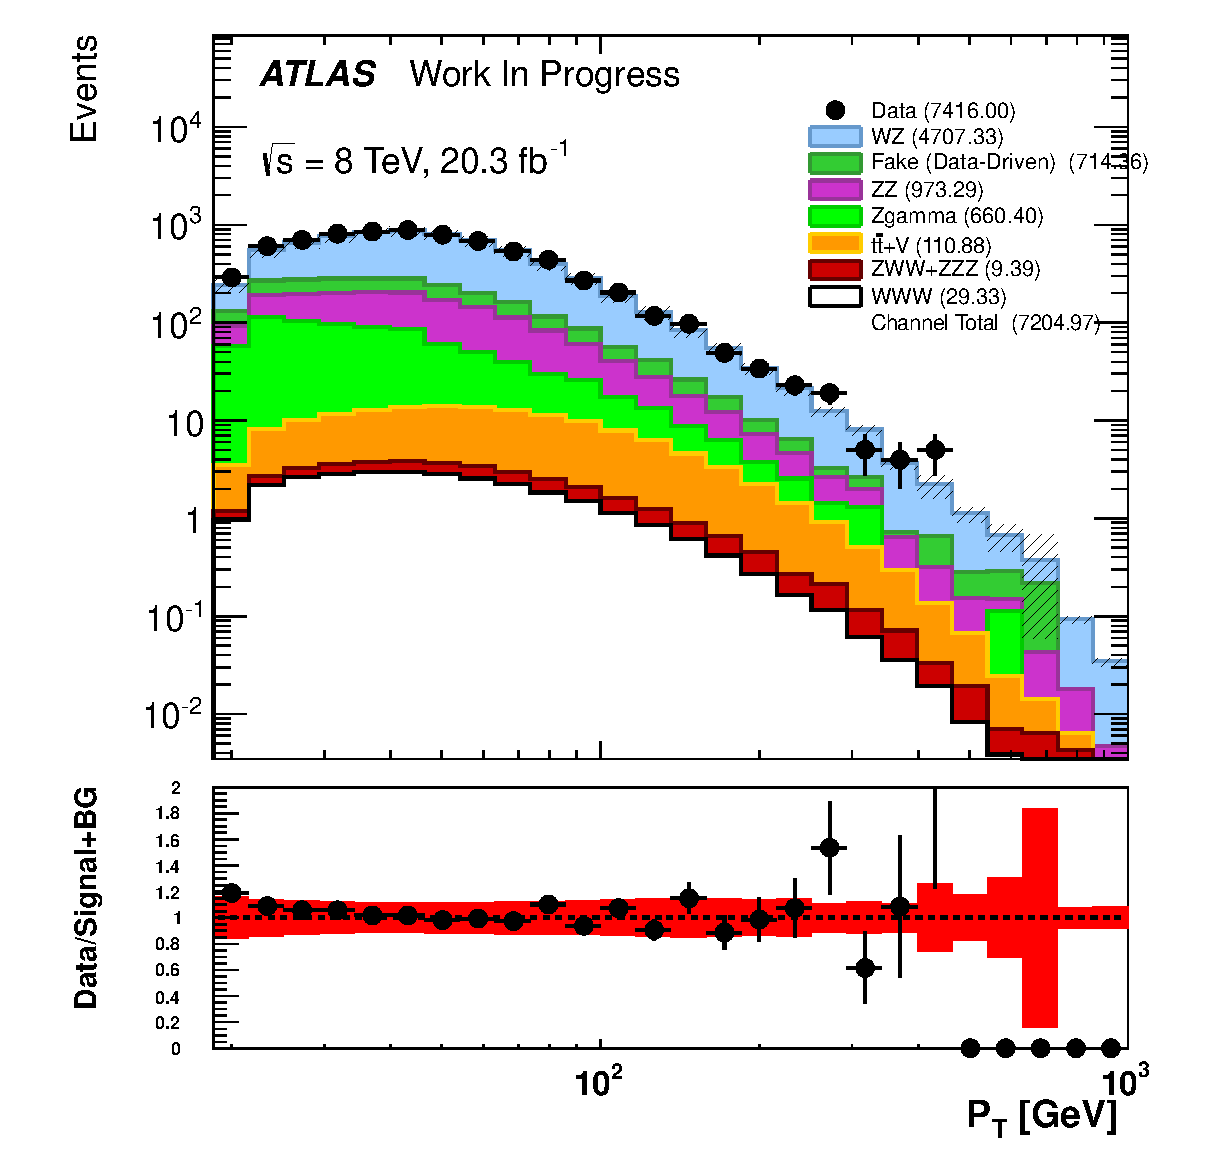
\includegraphics[width=0.3\textwidth]{figures/appendix_signal_selection/Nov24Update_FakeSys_KFacSys_LogY_NoRebin/output/jobs/MxM/DataFull_Rates_May13_FakeRatesExactly2Loose_MuonMxMBJetGt0_ElBJetGt0SubtractPC_MxM/PreselectionNov23_15_physics/weight_all/eps/AllLeptonPt_histratio.eps}
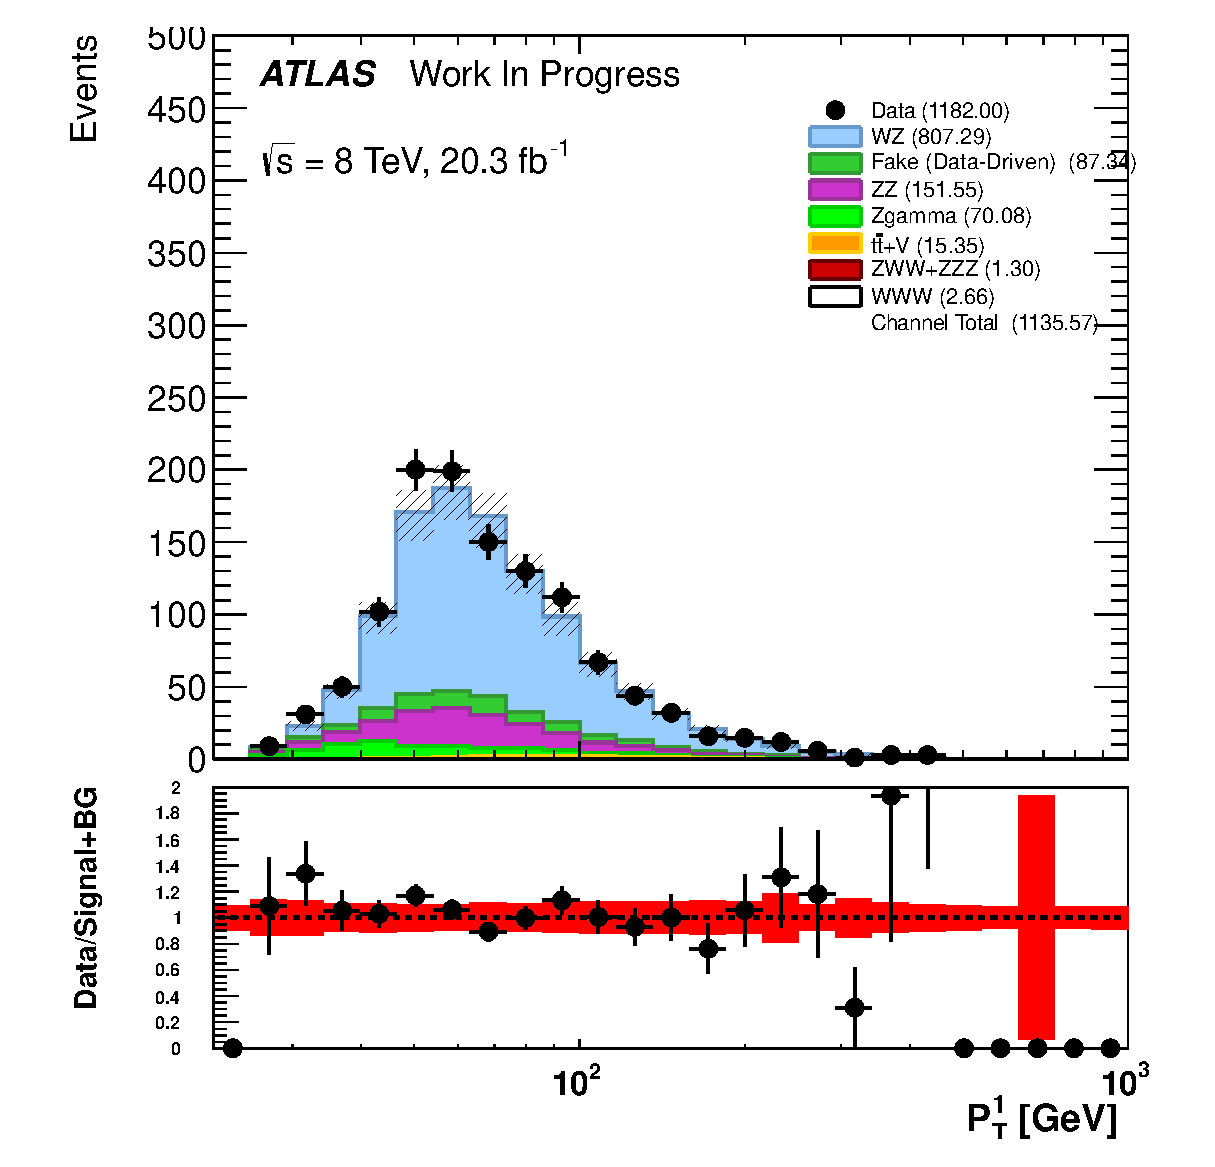
\includegraphics[width=0.495\textwidth]{figures/appendix_signal_selection/Nov24Update_FakeSys_KFacSys_LogY_NoRebin/output/jobs/MxM/DataFull_Rates_May13_FakeRatesExactly2Loose_MuonMxMBJetGt0_ElBJetGt0SubtractPC_MxM/PreselectionNov23_15_physics/weight_all/eps/LeadingLeptonPt_histratio.eps}
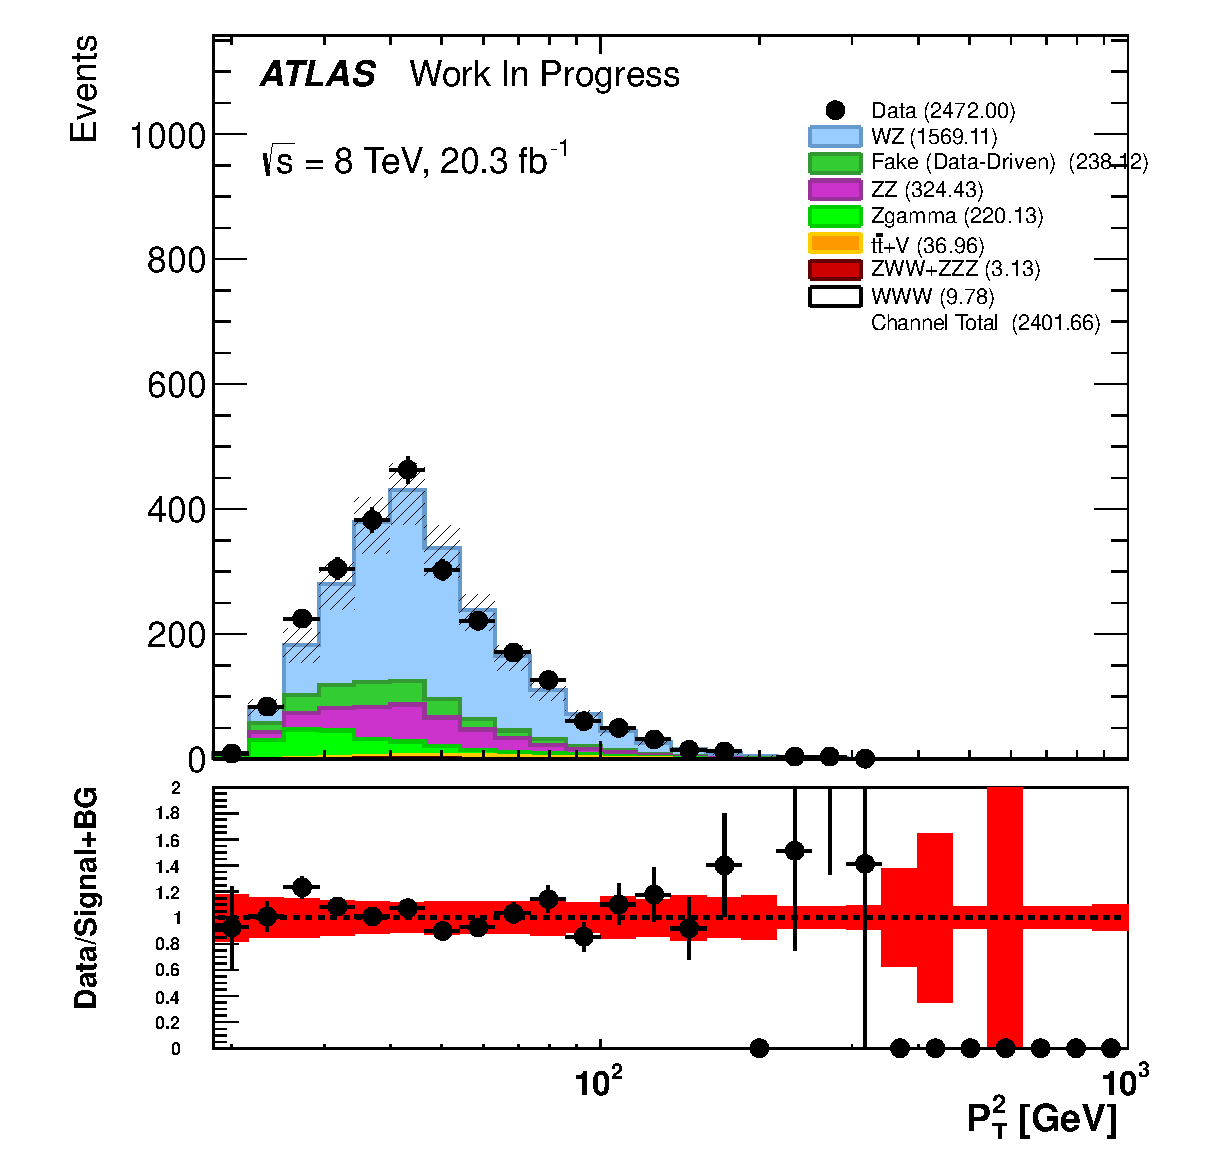
\includegraphics[width=0.495\textwidth]{figures/appendix_signal_selection/Nov24Update_FakeSys_KFacSys_LogY_NoRebin/output/jobs/MxM/DataFull_Rates_May13_FakeRatesExactly2Loose_MuonMxMBJetGt0_ElBJetGt0SubtractPC_MxM/PreselectionNov23_15_physics/weight_all/eps/SubleadingLeptonPt_histratio.eps}
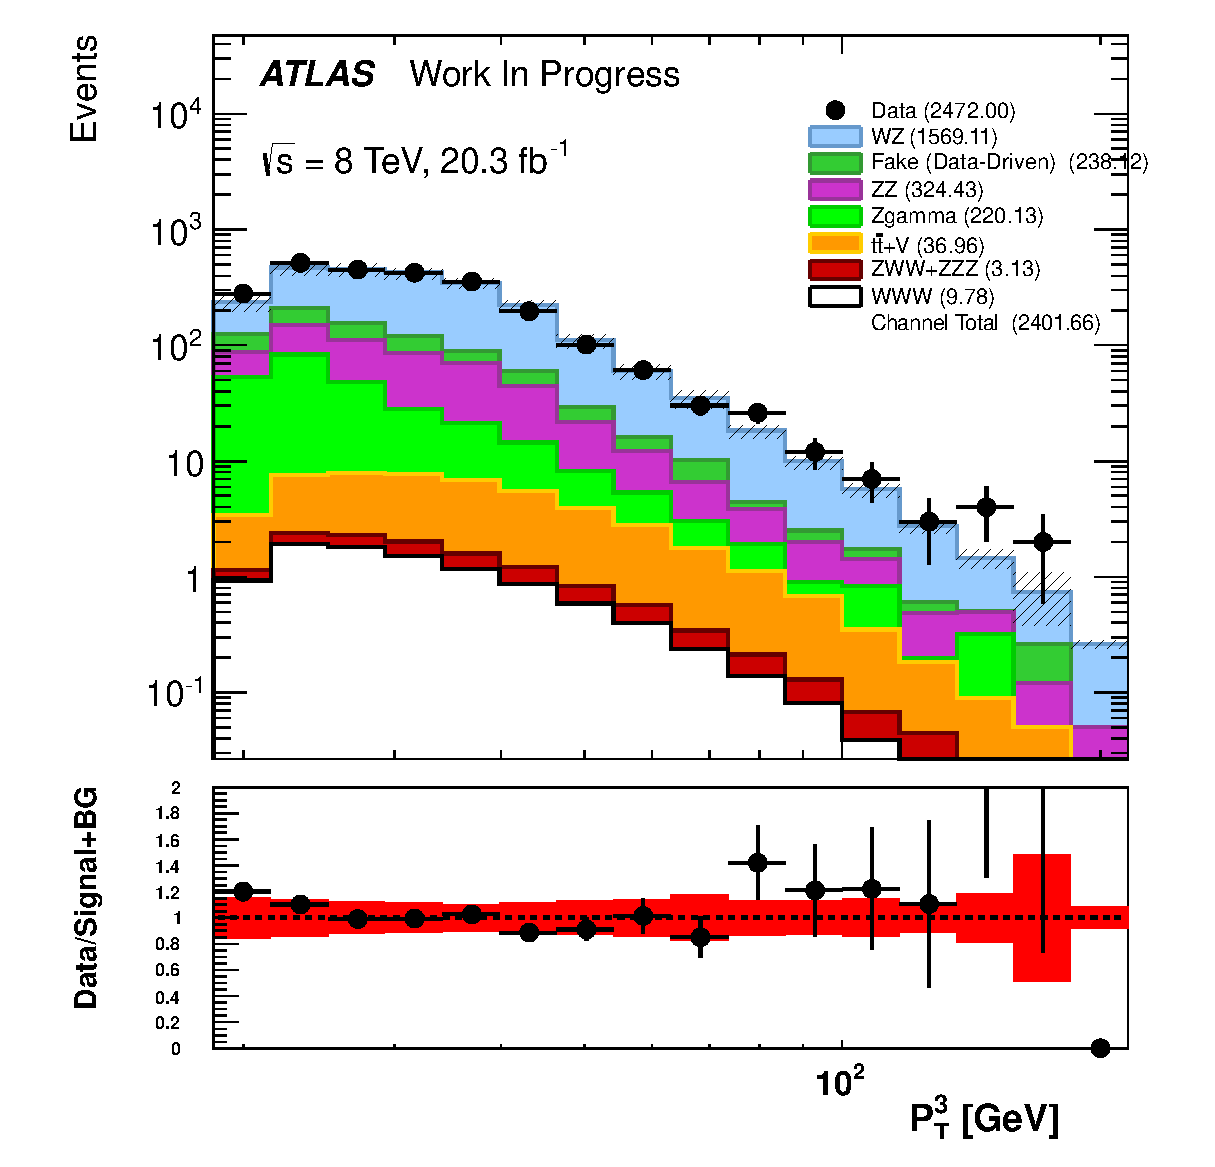
\includegraphics[width=0.495\textwidth]{figures/appendix_signal_selection/Nov24Update_FakeSys_KFacSys_LogY_NoRebin/output/jobs/MxM/DataFull_Rates_May13_FakeRatesExactly2Loose_MuonMxMBJetGt0_ElBJetGt0SubtractPC_MxM/PreselectionNov23_15_physics/weight_all/eps/MinimumLeptonPt_histratio.eps}
\includegraphics[width=0.495\textwidth]{figures/appendix_signal_selection/Nov24Update_FakeSys_KFacSys_LogY_NoRebin/output/jobs/MxM/DataFull_Rates_May13_FakeRatesExactly2Loose_MuonMxMBJetGt0_ElBJetGt0SubtractPC_MxM/PreselectionNov23_15_physics/weight_all/eps/MET_Et_histratio.eps}
%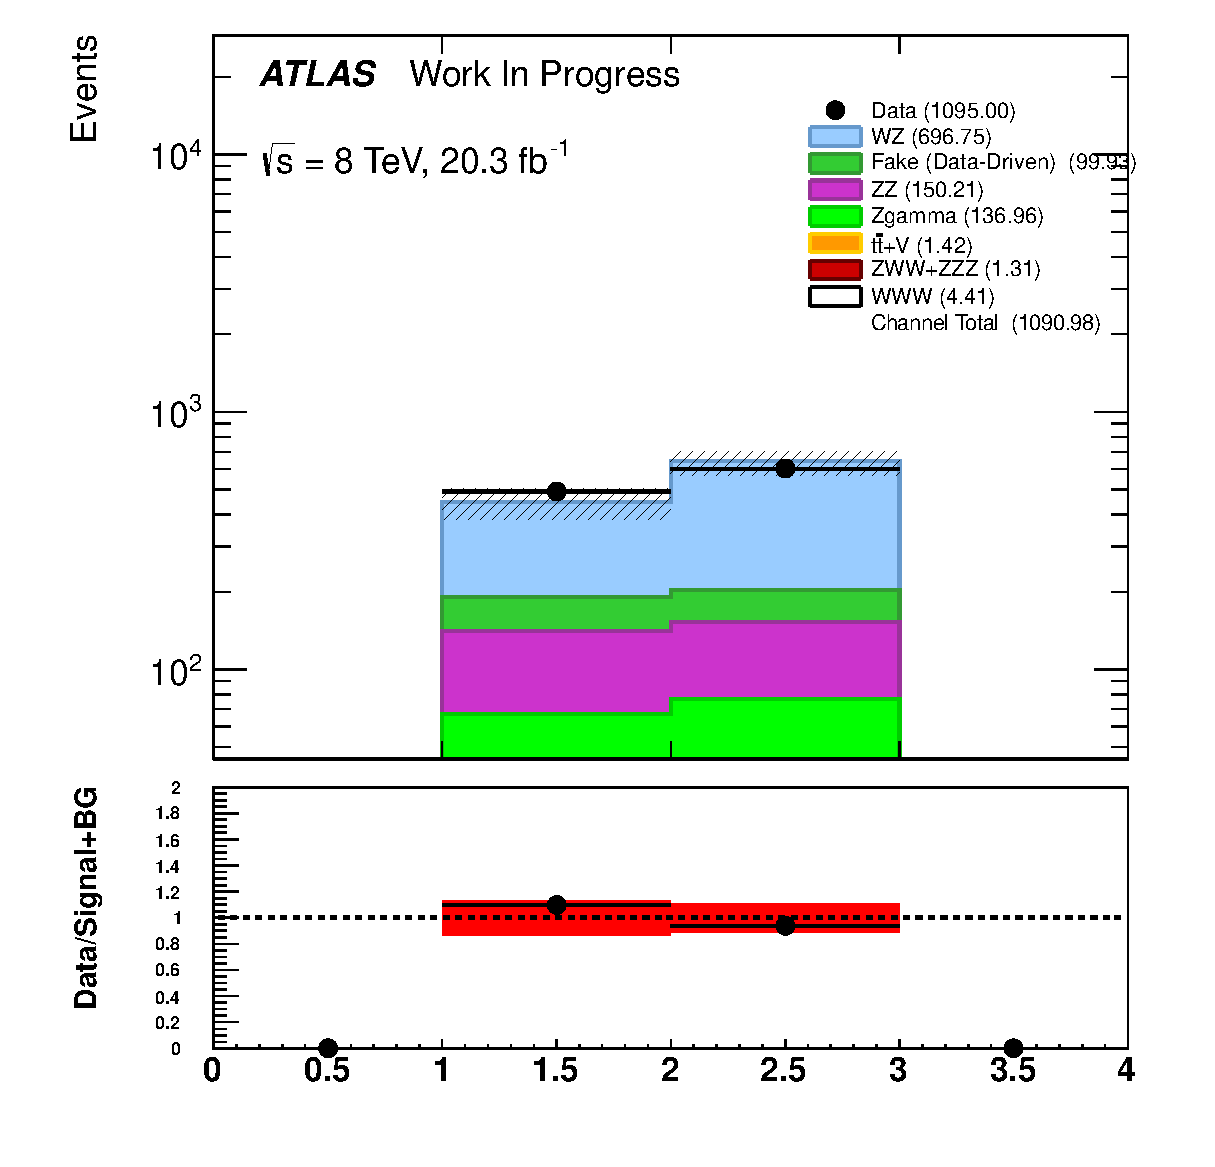
\includegraphics[width=0.3\textwidth]{figures/appendix_signal_selection/Nov24Update_FakeSys_KFacSys_LogY_NoRebin/output/jobs/MxM/DataFull_Rates_May13_FakeRatesExactly2Loose_MuonMxMBJetGt0_ElBJetGt0SubtractPC_MxM/PreselectionNov23_15_physics/weight_all/eps/TotalCharge_histratio.eps}
\caption{Distributions showing the observed data compared to the background estimate at event pre-selection.
From top to bottom and left to right, these distributions are: the leading, 
sub-leading, and minimum lepton \pt~(ordered by their \pt), 
\MET.
}
\label{fig:preselection1}
\end{figure}

\begin{figure}[htb]
\centering
%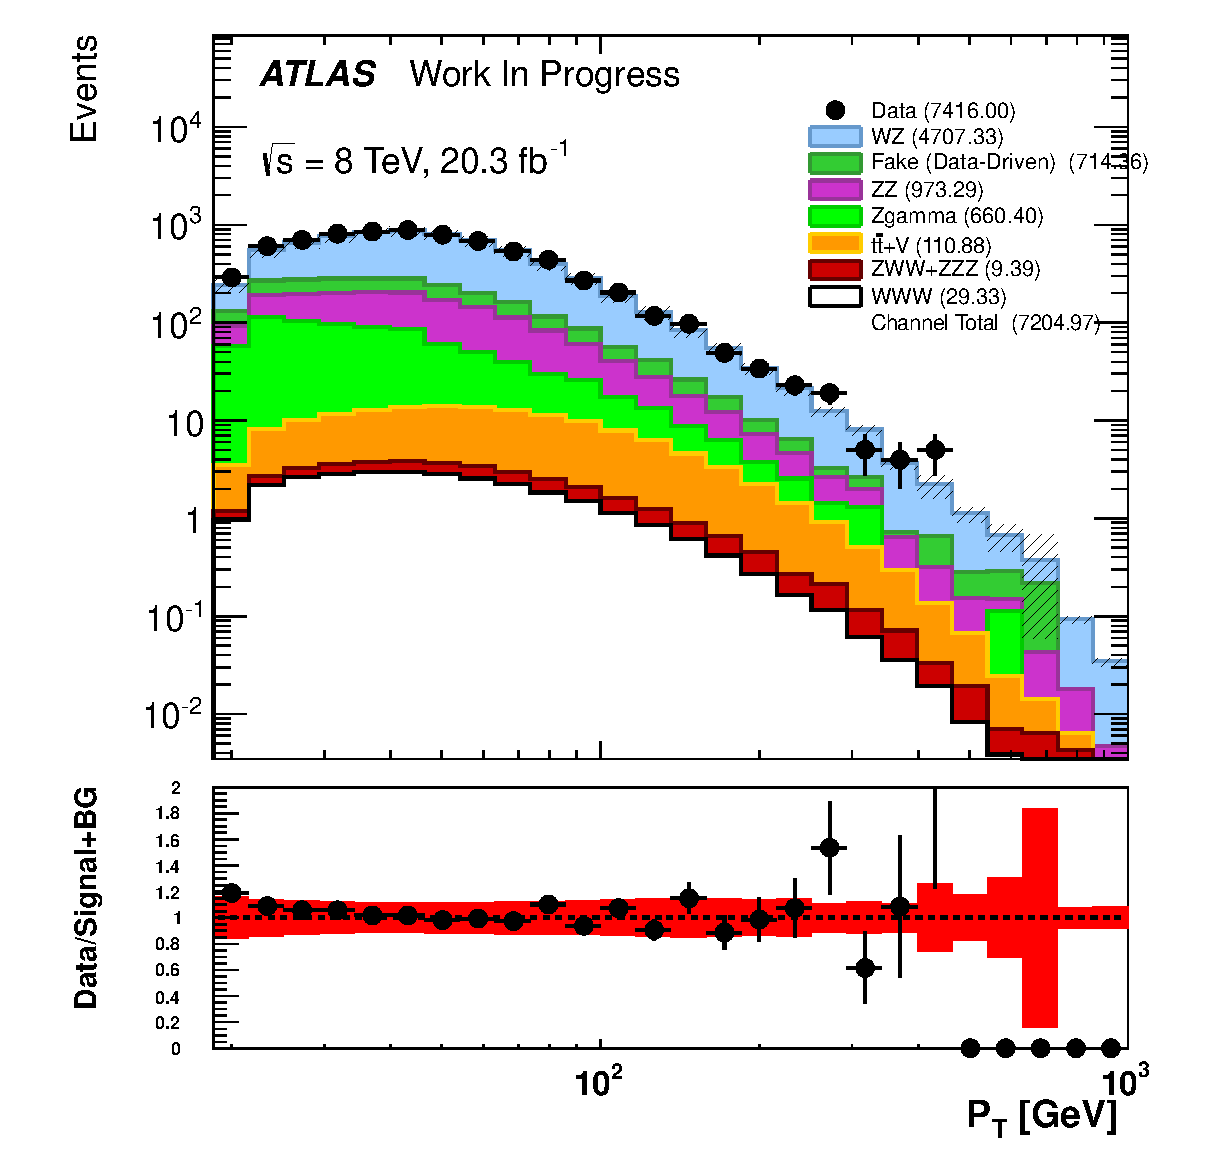
\includegraphics[width=0.3\textwidth]{figures/appendix_signal_selection/Nov24Update_FakeSys_KFacSys_LogY_NoRebin/output/jobs/MxM/DataFull_Rates_May13_FakeRatesExactly2Loose_MuonMxMBJetGt0_ElBJetGt0SubtractPC_MxM/PreselectionNov23_15_physics/weight_all/eps/AllLeptonPt_histratio.eps}
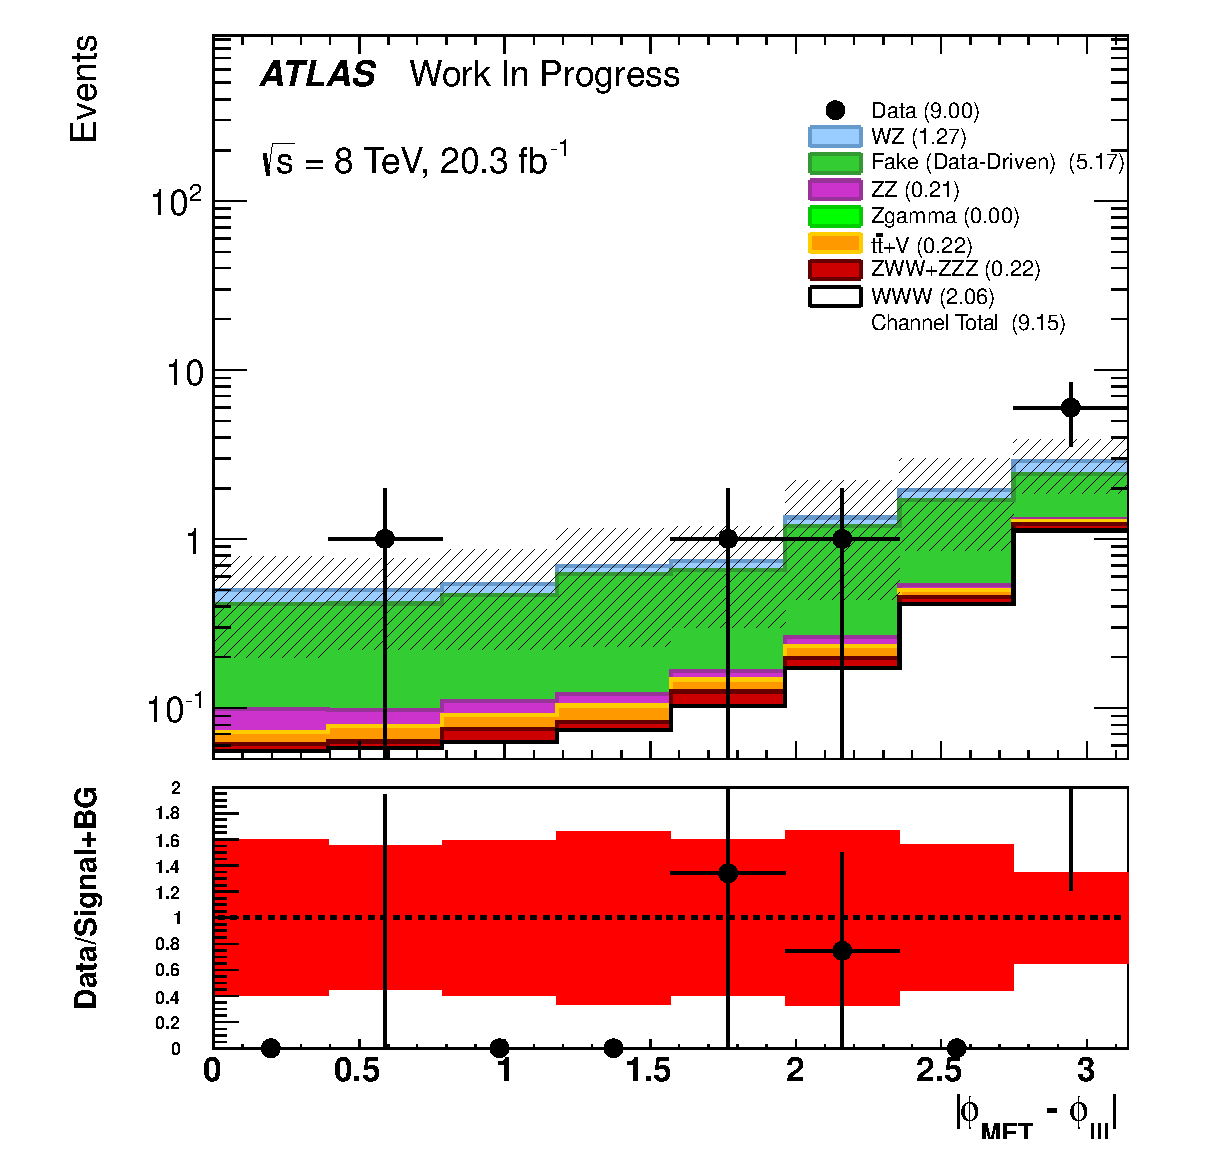
\includegraphics[width=0.495\textwidth]{figures/appendix_signal_selection/Nov24Update_FakeSys_KFacSys_LogY_NoRebin/output/jobs/MxM/DataFull_Rates_May13_FakeRatesExactly2Loose_MuonMxMBJetGt0_ElBJetGt0SubtractPC_MxM/PreselectionNov23_15_physics/weight_all/eps/DeltaPhiMET123_Abs_histratio.eps}
\includegraphics[width=0.495\textwidth]{figures/appendix_signal_selection/Nov24Update_FakeSys_KFacSys_LogY_NoRebin/output/jobs/MxM/DataFull_Rates_May13_FakeRatesExactly2Loose_MuonMxMBJetGt0_ElBJetGt0SubtractPC_MxM/PreselectionNov23_15_physics/weight_all/eps/InvariantMassSFOS_histratio.eps}
\includegraphics[width=0.495\textwidth]{figures/appendix_signal_selection/Nov24Update_FakeSys_KFacSys_LogY_NoRebin/output/jobs/MxM/DataFull_Rates_May13_FakeRatesExactly2Loose_MuonMxMBJetGt0_ElBJetGt0SubtractPC_MxM/PreselectionNov23_15_physics/weight_all/eps/NBTaggedJets_histratio.eps}
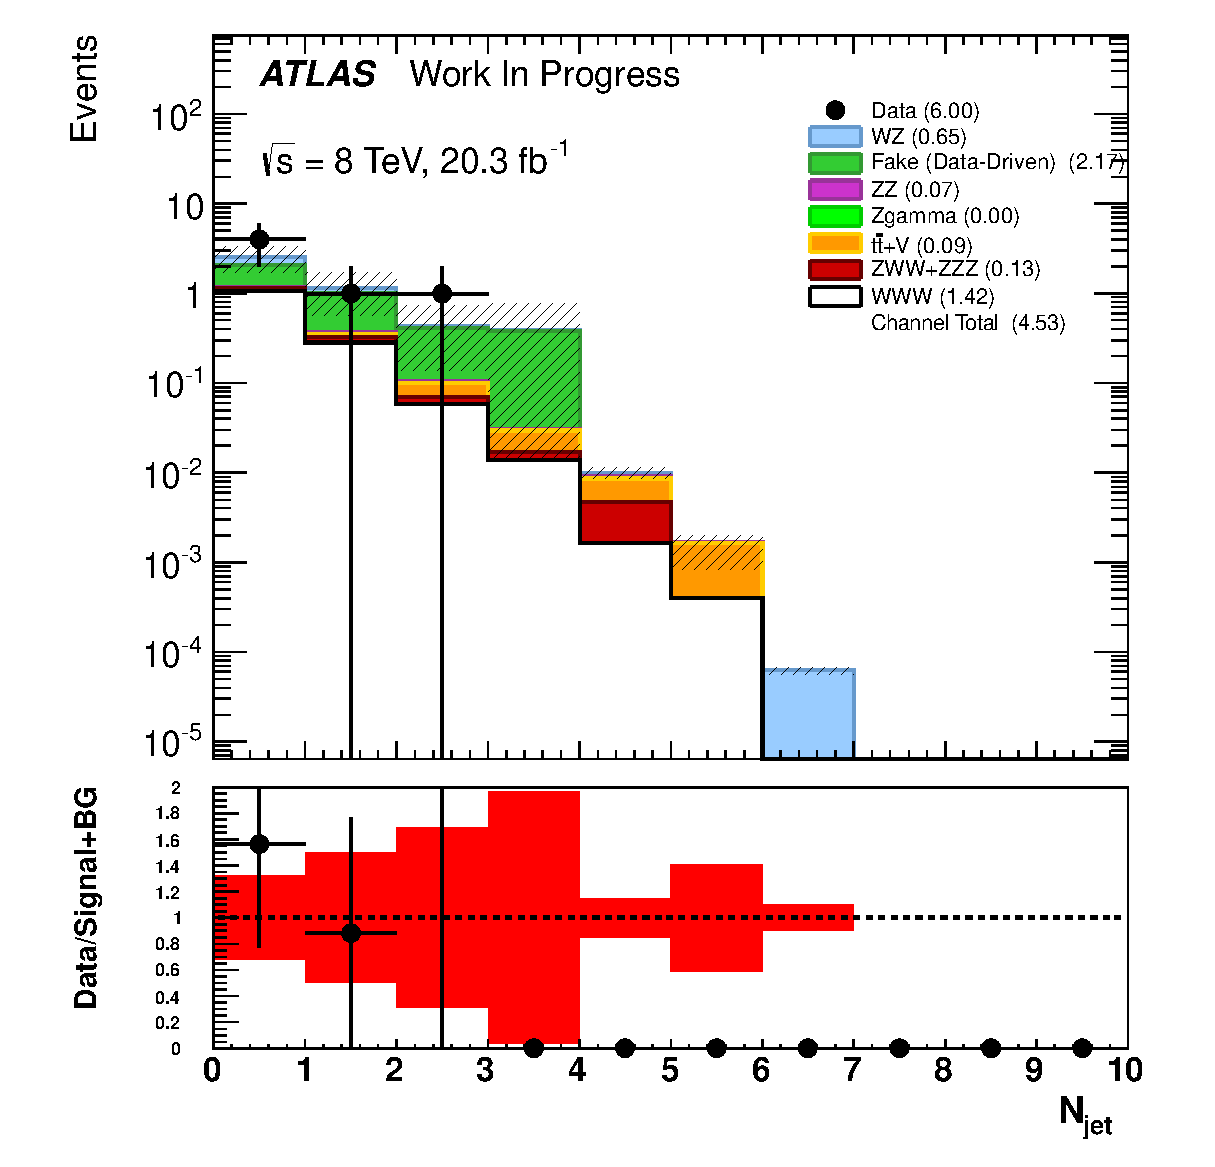
\includegraphics[width=0.495\textwidth]{figures/appendix_signal_selection/Nov24Update_FakeSys_KFacSys_LogY_NoRebin/output/jobs/MxM/DataFull_Rates_May13_FakeRatesExactly2Loose_MuonMxMBJetGt0_ElBJetGt0SubtractPC_MxM/PreselectionNov23_15_physics/weight_all/eps/NJets_histratio.eps}
%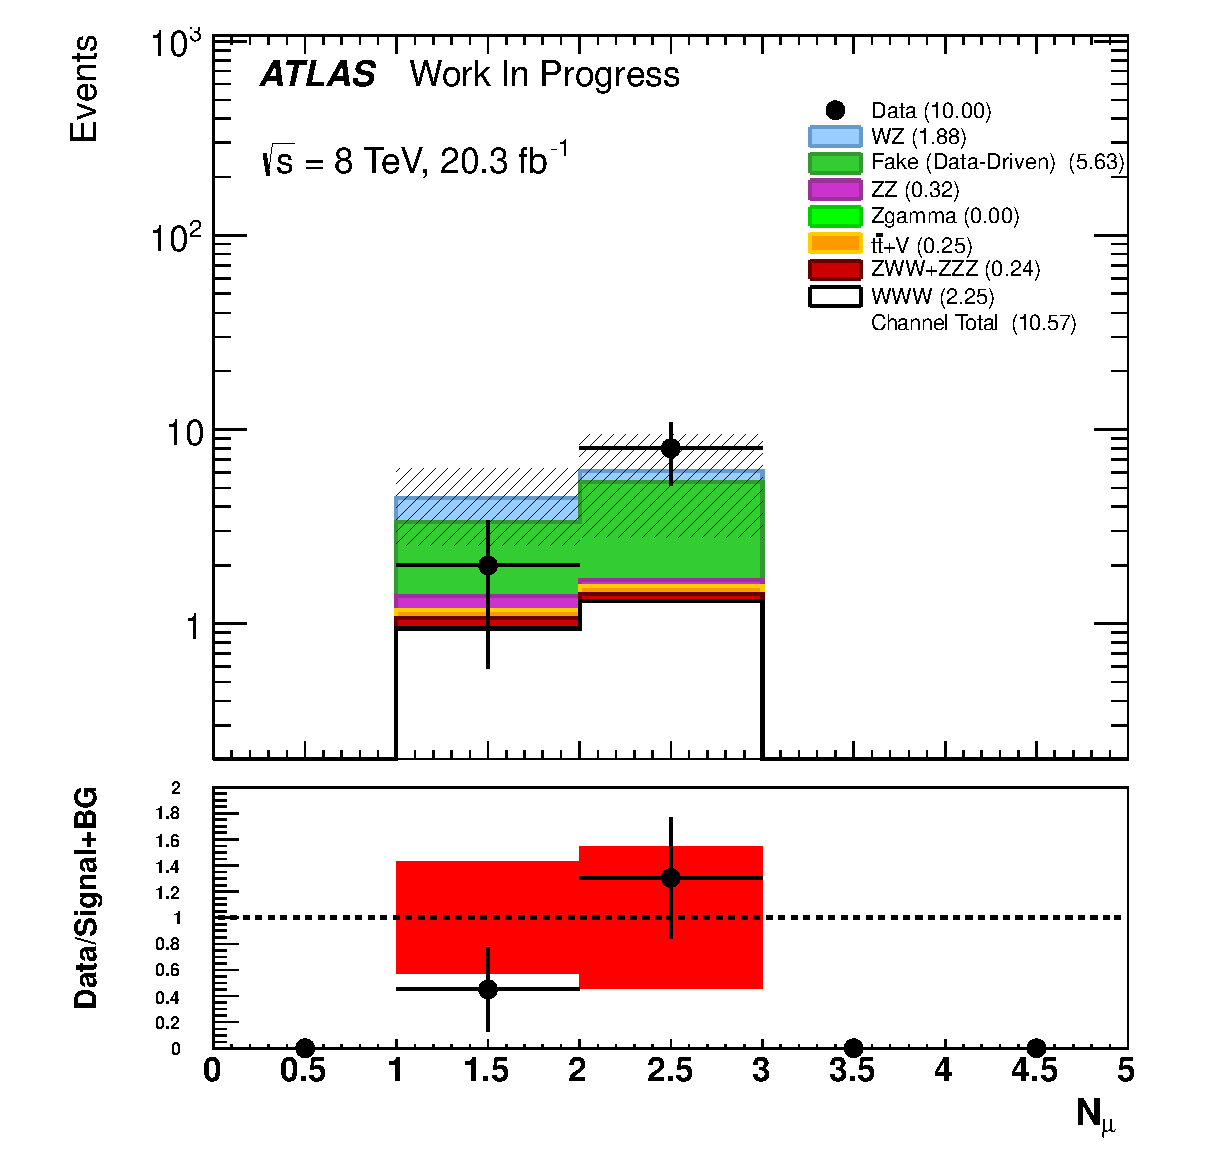
\includegraphics[width=0.495\textwidth]{figures/appendix_signal_selection/Nov24Update_FakeSys_KFacSys_LogY_NoRebin/output/jobs/MxM/DataFull_Rates_May13_FakeRatesExactly2Loose_MuonMxMBJetGt0_ElBJetGt0SubtractPC_MxM/PreselectionNov23_15_physics/weight_all/eps/NMuons_histratio.eps}
%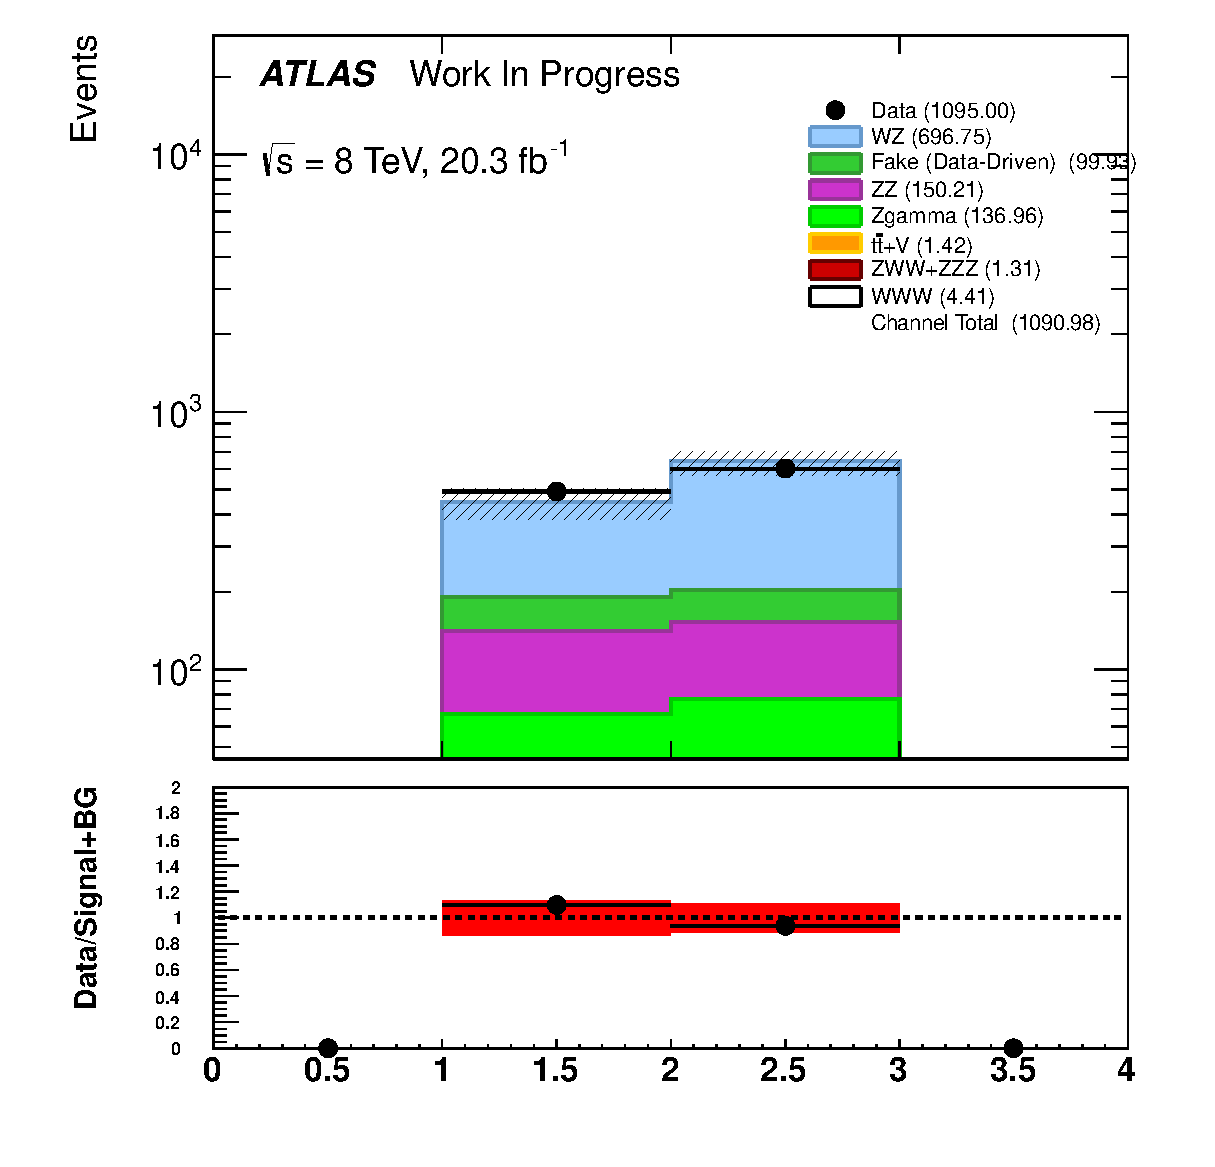
\includegraphics[width=0.3\textwidth]{figures/appendix_signal_selection/Nov24Update_FakeSys_KFacSys_LogY_NoRebin/output/jobs/MxM/DataFull_Rates_May13_FakeRatesExactly2Loose_MuonMxMBJetGt0_ElBJetGt0SubtractPC_MxM/PreselectionNov23_15_physics/weight_all/eps/TotalCharge_histratio.eps}
\caption{Distributions showing the observed data compared to the background estimate at event pre-selection.
From top to bottom and left to right, these distributions are: 
\deltaphi, $m_{\textrm{SFOS}}$, \njet, \nbjet, and $N_{\mu}$.
}
\label{fig:preselection2}
\end{figure}


The signal plus background model 
(described in detail in \sec\ref{sec:bg_estimates})
is compared to data at pre-selection, defined in \sec\ref{sec:preselection},
for a few different kinematic distributions 
in \fig\ref{fig:preselection1} and \fig\ref{fig:preselection2}. 
In the upper plot of each distribution,
the colored histograms 
represent the different categories contributing to the signal 
plus background model and 
are split by color based on the category. 
%The colors are...
Hashed bands are shown on the stacked
histograms representing the size of the systematic uncertainties 
on the model, described later in \sec\ref{sec:systematics}.
The data is shown in the black points where the 
bars on the points represent the statistical uncertainty on the data.
The lower plot shows the ratio of the data over the model.
The error bars correspond to the statistical uncertainty
on the ratio due to both the data and the model. The red band
shows the size of the systematic uncertainties with respect to the model.
The model is said to be consistent with the data
if the ratio is compatible with unity after considering statistical
and systematic uncertainties.
The different distributions are chosen primarily because 
of their potential to discriminate between signal and background. 
The number of signal events at pre-selection is predicted to be 
$9.78 \pm 0.041 \stat ^{+0.390}_{0.447} \syst$
while the number of predicted background events is 
$2387.9 \pm 6.5 \stat ^{+297.8}_{-285.2} \syst$. 
This is consistent with the 2472 events observed in the data.




%\begin{table}[ht!]
%\centering
%\begin{tabular}{|c||c|c|c|c|}
\hline
 & $eee$ & $ee\mu$ & $e\mu\mu$ & $\mu\mu\mu$\\ 
\hline\hline
$WZ$ &  $240.85 \pm 0.67$ &  $339.17 \pm 0.82$ &  $422.07 \pm 0.87$ &  $567.0 \pm 1$\\ 
$ZZ$ &  $60.21 \pm 0.13$ &  $54.1 \pm 0.2$ &  $118.60 \pm 0.31$ &  $91.48 \pm 0.17$\\ 
$Z\gamma$ &  $70.1 \pm 2.7$ &  $0.47 \pm 0.22$ &  $149.4 \pm 3.9$ &  $0.17 \pm 0.12$\\ 
$ZWW+ZZZ$ &  $0.436 \pm 0.019$ &  $0.834 \pm 0.027$ &  $1.00 \pm 0.03$ &  $0.864 \pm 0.028$\\ 
$t\bar{t}+V$ &  $4.854 \pm 0.044$ &  $9.549 \pm 0.064$ &  $12.047 \pm 0.072$ &  $10.510 \pm 0.066$\\ 
Fake (data-driven) &  $45.1 \pm 2.2$ &  $37.8 \pm 1.6$ &  $112.7 \pm 2.8$ &  $42.5 \pm 1.2$\\ 
$WWW$ &  $0.770 \pm 0.011$ &  $3.023 \pm 0.023$ &  $3.970 \pm 0.026$ &  $1.843 \pm 0.018$\\ 
\hline
Expected Background &  $421.6 \pm 3.5$ &  $441.9 \pm 1.8$ &  $815.8 \pm 4.9$ &  $712.5 \pm 1.6$\\ 
Expected Signal + Background &  $422.4 \pm 3.5$ &  $444.9 \pm 1.8$ &  $819.8 \pm 4.9$ &  $714.4 \pm 1.6$\\ 
\hline
Observed Data &  $426 \pm 21$ &  $468 \pm 22$ &  $821 \pm 29$ &  $757 \pm 28$\\ 
\hline
\end{tabular}

%\caption{Expected and observed event yields binned by lepton flavor combination at event pre-selection.
%Only statistical uncertainties are shown.
%}
%\label{tab:preselection}
%\end{table}



\begin{figure}[ht!]
\centering
\includegraphics[width=0.8\textwidth]{figures/SFOSPreselection.png}
\caption{Yields at event pre-selection in the 0, 1 and 2 SFOS regions.  
The most important systematic uncertainties 
(discussed in section~\ref{sec:systematics}) are shown, 
namely from the fake estimates and the uncertainties on the WZ and ZZ k-factors.}
\label{fig:preselection_nsfos}
\end{figure}

Upon splitting the pre-selection region based on the number of SFOS
pairs, we end up with the signal and background predictions in
\fig\ref{fig:preselection_nsfos}, where we can see differences
in the branching fraction for the signal to fall into
each of the three signal regions.
In the 0 and 2 SFOS regions, roughly 2.5 signal events are predicted
whereas closer to 5 signal events are predicted in the 1 SFOS region.
Shifting to looking at the background, perhaps the most striking 
feature of this plot is the 
clear difference in background yield and background composition
between the 0 SFOS region and the 1 and 2 SFOS regions.
More than 1000 background events are predicted in both the 1 and
the 2 SFOS regions, but only about 30 background events are
predicted in the 0 SFOS region.
Clearly then, the advantage of splitting the signal region based on this
classification comes when looking at the background, specifically the
electroweak $WZ$ and $ZZ$ backgrounds where SFOS lepton pairs may be
produced from the decay of the $Z$ boson(s). Consider only the case
where the $WZ$ and $ZZ$ decay to either electrons or muons.  The $WZ$ production
process is thus characterized by 3 leptons with at least 1 SFOS lepton pair
that comes from the $Z$. If all three leptons from the $WZ$ decay have been
reconstructed, then there is a 50~\% chance the third lepton 
will also be able to form a SFOS pair with one of the leptons from the $Z$ decay.
Thus, the WZ background will split evenly between the 1 and 2 SFOS classification.
Something similar occurs for the ZZ background except that the fourth lepton 
in the decay must be lost (usually due to possessing a low $\pt$).
The large cross-section for these processes means that
they become the dominant backgrounds in the 1 and 2 SFOS regions.  
The 0 SFOS signal region is mostly spared from contamination  by 
these large processes but still
includes both the $WZ$ and $ZZ$ processes as background due to the
non-negligible (albeit small) effect of mis-measurement of the electron
charge described in \sec\ref{sec:charge_misid} and the presence
of leptonically decaying taus.  The 0 SFOS signal region
is thus unique in having a small background which is almost entirely
reducible and dominated instead by the fake background,
described in \sec\ref{sec:bg_fake},
along with contamination from $WZ$ and $ZZ$. 
\FloatBarrier

\subsection{Optimization}
\label{sec:optimization}
From the above discussion, one can clearly see that it is
advantageous to split these signal regions so that the dominant
backgrounds in each region may be targeted individually.  Furthermore,
note that even though the 1 SFOS region contains more of the signal than the
0 and 2 SFOS regions, it is the 0 SFOS region which is most likely to
have the best sensitivity due to the smaller background contribution.
In \sec\ref{sec:signal_regions} it was already shown
that a selection was chosen based on an optimization procedure
designed to further reduce the background with respect to the 
signal region. 

The optimization takes as input a multi-dimensional 
space where each dimension is the selection threshold
for one of the quantities listed in \tab\ref{tab:signal_selection}, 
plus some others.
The range of the multi-dimensional space 
is restricted so that the 
predicted signal remains finite i.e. non-zero.
At an individual point in this space, the optimization computes
the expected signal and background events after the selection
along with the size of statistical uncertainties
and systematic uncertainties on the model. 
These are then used as input to the measurement extraction framework
described in \sec\ref{sec:measurement} to determine the width of the precision
on the final measurement. 
This width is used as the metric to minimize in the optimization.
By considering a metric like this, we are optimizing directly
the quantity of interest to the final measurement, and taking
into account not just the individual predictions, but also their
uncertainties. This is important because it can more stringently
remove backgrounds that have large uncertainties.

We choose to treat the sample space as being discrete as opposed
to continuous. For some dimensions of the space, such as 
the threshold on \njet, this is manifestly true, as there 
can only be an integer number of observed jets. 
For other dimensions, such as the threshold on the lepton
\pt, these quantities are real valued and thus continuous.
%looking at \fig\ref{fig:optimization_efficiencies_preselection} 
%and \fig\ref{fig:optimization_efficiencies_0sfos}, 
%the shape of the efficiencies tend to change relatively slowly from bin to bin 
It should be acceptable to only sample 
discretely, however,  as long as they can capture the shape information of 
the efficiencies. % as they do above. 
Furthermore, 
this acknowledges the finite  experimental resolution of these 
quantities. For example,
the difference between $\pt > 20~\GeV$ and $\pt > 20.5~\GeV$
should not be taken too seriously because of the effects of limited
track and energy resolution used to derive the muon and electron \pt.
%expand on this? what would be the typical electron and muon resolution here?
Treating the sample space as discrete means that the optimization
function is not smooth and so cannot readily take into account
derivative information to be used for instance 
in some sophisticated minimization algorithm.
Fortunately, the number of points in the sample space after discretizing, 
though large, is small enough that it can be evaluated in its entirety
using a brute force approach. Thus, we choose to evaluate the 
optimization in the restricted and discretized sample space in order
to find an optimal choice for the selection.

%I should redo the optimization for the specific bin sizes and list them

The shape of the optimization can be seen in \fig\ref{fig:optimization}.
\emph{Figures need to be reproduced. Elaborate...} 


\begin{figure}[ht!]
\centering

\includegraphics[width=0.3\columnwidth]{figures/placeholder.eps}

\includegraphics[width=0.3\columnwidth]{figures/placeholder.eps}

\includegraphics[width=0.3\columnwidth]{figures/placeholder.eps}
\caption{Signal Yield vs Measurement Uncertainty for optimized points 
in the 0 SFOS (left), 1 SFOS (middle), and 2 SFOS (right) signal regions.}
\label{fig:optimization}
\end{figure}


The final selection is presented in \tab\ref{tab:signal_selection}.
Details of the specific cut thresholds that are chosen can be understood
by looking closer at some of the quantities used as input to 
the optimization. For instance, it is observed that
different \MET~and \z-veto thresholds are chosen for the 1 and 2 SFOS
regions. This can be understood to come from a correlation between
these two quantities due to their ability to isolate the $Z\gamma$
background.
The $Z\gamma$ background shows up in the low-shoulder of the \z-peak
in the $m_{\textrm{SFOS}}$ distribution and at low MET. This can be
seen both for the 1 and 2 SFOS regions in \fig\ref{fig:met_zwindow_optimization}.
As a result, the $Z\gamma$ background can be removed either by tuning 
the \z-mass window used in the veto above, or by removing events with low \met.
Thus, the optimization shows that there is some correlation 
between the \z-veto window and the \met~selection threshold. 
In the 1 SFOS region, there is a larger 
contribution from $Z\gamma$ processes than in the 2 SFOS
region.  This process mostly shows up in the low shoulder 
of the \z~ peak. The optimization
prefers removing this $Z\gamma$ contribution by setting an 
asymmetric \z-window in the 1 SFOS
region, with the boundaries being 35~GeV below the \z-pole 
and 20~GeV above and then keeping the \MET~cut a little loose, with a 
threshold of $\MET > 45$~GeV.  In the 2 SFOS region, however,
the $Z\gamma$ contribution is not as prominent and the 
optimization happens to prefer a symmetric
window of $\pm20$~GeV around the \z-pole.  
The looser \z-veto then allows for a tighter
missing $E_{T}$ cut with a threshold of $\MET > 55$~GeV. 

\begin{figure}[ht!]
\centering
\includegraphics[width=0.4\columnwidth]{figures/appendix_signal_selection/Nov24Update_FakeSys_KFacSys_LogY_NoRebin/output/jobs/MxM/DataFull_Rates_May13_FakeRatesExactly2Loose_MuonMxMBJetGt0_ElBJetGt0SubtractPC_MxM/PreselectionNov23_15_1SFOS_ChargeAbs1_BVeto85_physics/weight_all/png/MET_Et_histratio.png}
\includegraphics[width=0.4\columnwidth]{figures/appendix_signal_selection/Nov24Update_FakeSys_KFacSys_LogY_NoRebin/output/jobs/MxM/DataFull_Rates_May13_FakeRatesExactly2Loose_MuonMxMBJetGt0_ElBJetGt0SubtractPC_MxM/PreselectionNov23_15_1SFOS_ChargeAbs1_BVeto85_physics/weight_all/png/InvariantMassSFOS_histratio.png}
\includegraphics[width=0.4\columnwidth]{figures/appendix_signal_selection/Nov24Update_FakeSys_KFacSys_LogY_NoRebin/output/jobs/MxM/DataFull_Rates_May13_FakeRatesExactly2Loose_MuonMxMBJetGt0_ElBJetGt0SubtractPC_MxM/PreselectionNov23_15_2SFOS_ChargeAbs1_BVeto85_physics/weight_all/png/MET_Et_histratio.png}
\includegraphics[width=0.4\columnwidth]{figures/appendix_signal_selection/Nov24Update_FakeSys_KFacSys_LogY_NoRebin/output/jobs/MxM/DataFull_Rates_May13_FakeRatesExactly2Loose_MuonMxMBJetGt0_ElBJetGt0SubtractPC_MxM/PreselectionNov23_15_2SFOS_ChargeAbs1_BVeto85_physics/weight_all/png/InvariantMassSFOS_histratio.png}
\caption{Plots of the \MET (left) and $m_{\textrm{SFOS}}$ (right) distributions 
in the 1 SFOS (top) and 2 SFOS (bottom) regions after pre-selection
plus the \bee-veto requirement.}
\label{fig:met_zwindow_optimization}
\end{figure}

The absence of any cut on the \MET~distribution in the 0 SFOS
region can be better understood by looking at the 
the efficiency for selection between 
the signal and the background as a function of the \MET~selection threshold.
This is shown in \fig\ref{fig:met_eff} both after pre-selection
and in the 0 SFOS region.
Clearly, the signal efficiency closely follows the background efficiency
in the 0 SFOS region. Thus, there is no change in the
signal-to-background ratio when cutting on the \MET~distribution
in the 0 SFOS region and thus no improvement in the sensitivity.
On the other hand, there are large shape differences 
between the signal
and background efficiencies at pre-selection, with the 
signal efficiency remaining flatter at low values of the \MET~
threshold. So, from this one would expect a selection
on the \MET~threshold to be useful in the 1 and 2 SFOS
regions which have a similar background composition. 
Indeed, this is what we observe.


\begin{figure}[ht!]
\centering
\includegraphics[width=0.45\columnwidth]{figures/optimization/SignalRegionsPreselection_0SFOS_Efficiencies/MET_Et_STVF_Cumulative.eps}
\includegraphics[width=0.45\columnwidth]{figures/optimization/SignalRegions_0p5mmZ0_Preselection_Efficiencies/MET_Et_STVF_Cumulative.eps}
\caption{ Signal and background efficiencies for the 
selection $\MET > X$ as a function of the \MET~selection
threshold, $X$,  in both the 0 SFOS (left) and pre-selection (right) regions.  }
\label{fig:met_eff}
\end{figure}

The threshold for the jet multiplicity cut 
of $\njet\leq 1$ applied in all signal regions
is also determined from the optimization. One might expect
that a different value for the threshold, such as a complete
veto on the presence of jets, would perform better. 
Indeed, looking at the efficiency for selection on the jet multiplicity
in \fig\ref{fig:njet_eff} does show a much stronger background
rejection when applying a veto in both the pre-selection region
and especially in the 0 SFOS region where there is a larger
contribution from fakes due to hadronic activity.
The signal rejection, however,  of about 40\% observed in both
regions, is prohibitive. Loosening the selection to the nominal
threshold of $\njet \leq 1$ instead preserves 90\% of the signal, 
which is quite precious.  We are still able to remove 
much of the fake background in the 0 SFOS region by vetoing
events with \bee-tagged jets as can be seen in \fig\ref{fig:nbjet_eff}.
%any mention of different operating points
It is possible that using a \bee-tagging operating point
with an even higher \bee-tagging efficiency would further 
improve the sensitivity in the 0 SFOS region.  
The nominal operating point used here, however,  is the highest 
efficiency operating point supported by ATLAS.
Clearly, there is no advantage gained from using a looser operating point
as this would only cut less on the background without having an impact
on the signal.



\begin{figure}[ht!]
\centering
\includegraphics[width=0.45\columnwidth]{figures/optimization/SignalRegionsPreselection_0SFOS_Efficiencies/NJets_LeftCumulative.eps}
\includegraphics[width=0.45\columnwidth]{figures/optimization/SignalRegions_0p5mmZ0_Preselection_Efficiencies/NJets_LeftCumulative.eps}
\caption{ Signal and background efficiencies for the selection
$\njet \leq X$ as a function of the \njet~selection
threshold, $X$, in both the 0 SFOS (left) and pre-selection (right) regions.  }
\label{fig:njet_eff}
\end{figure}

\begin{figure}[ht!]
\centering
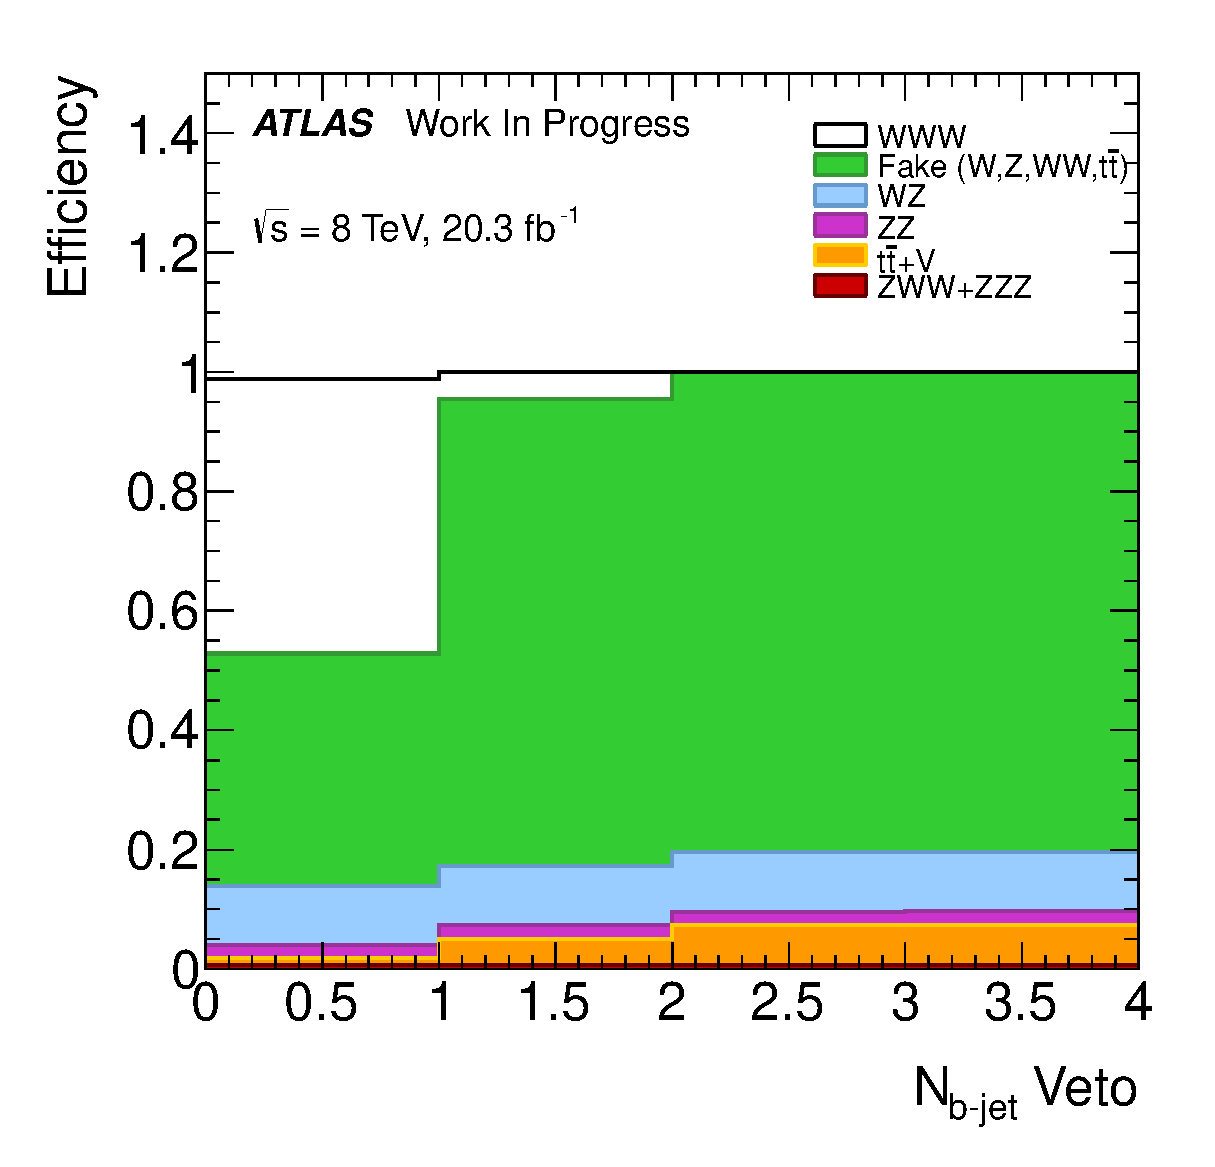
\includegraphics[width=0.45\columnwidth]{figures/optimization/SignalRegionsPreselection_0SFOS_Efficiencies/NBTaggedJets_LeftCumulative.eps}
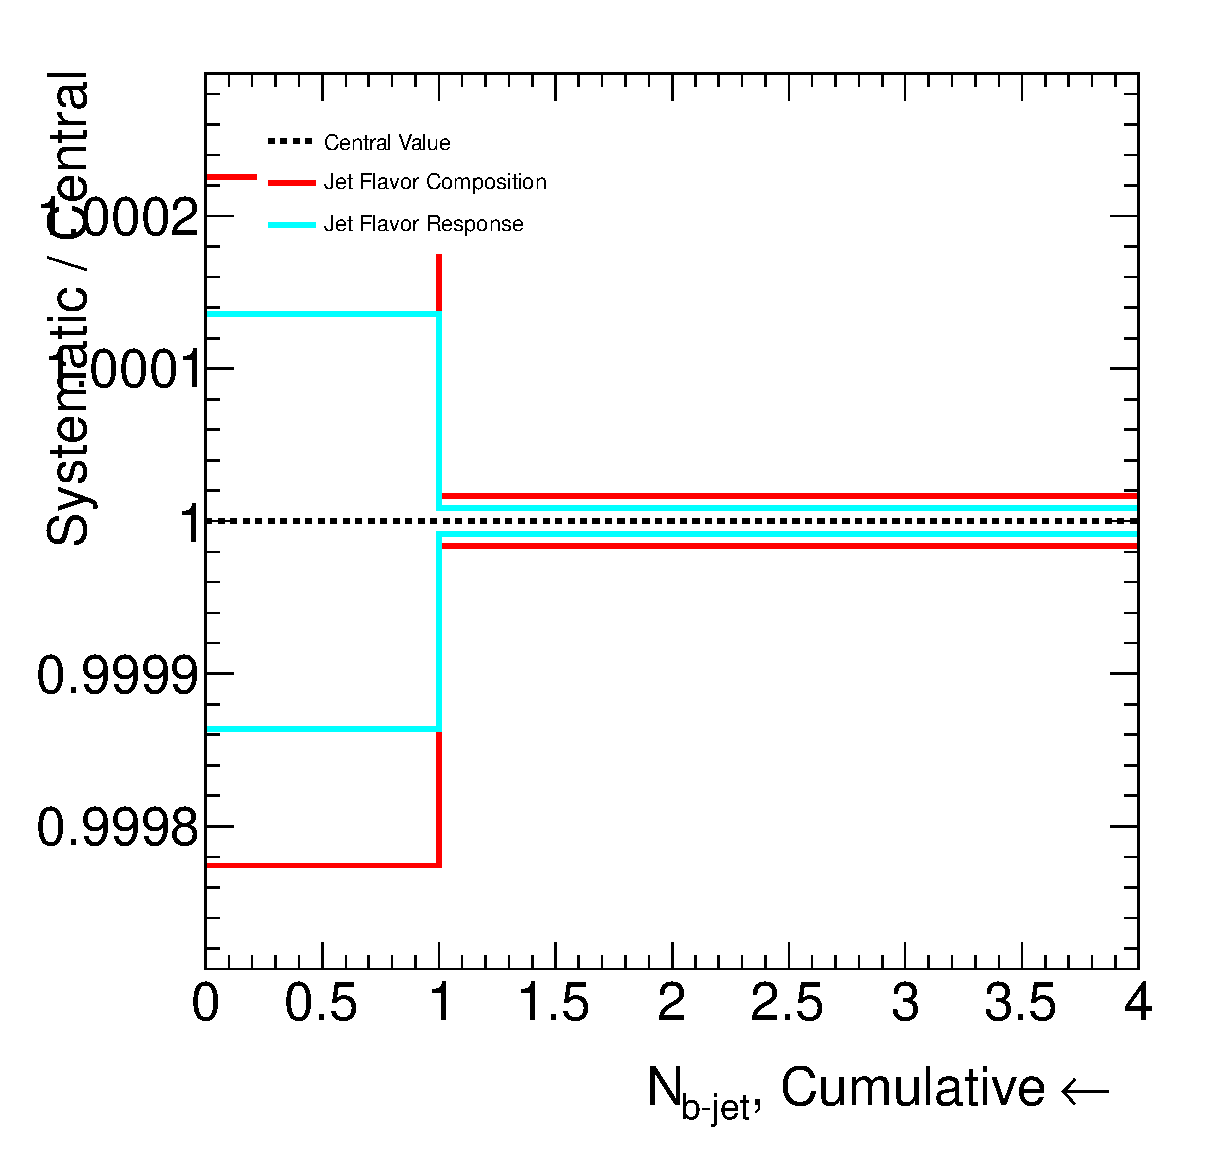
\includegraphics[width=0.45\columnwidth]{figures/optimization/SignalRegions_0p5mmZ0_Preselection_Efficiencies/NBTaggedJets_LeftCumulative.eps}
\caption{ Signal and background efficiencies 
for the selection
$\nbjet \leq X$
as a function of the \nbjet~selection
threshold, $X$, in both the 0 SFOS (left) and pre-selection (right) regions.  }
\label{fig:nbjet_eff}
\end{figure}


The \deltaphi~distribution for the signal is observed to be more back-to-back
(i.e. closer to $\pi$)
than that for the background. This is especially true in the 0 SFOS
region, as can be seen from the efficiencies plotted 
as a function of the \deltaphi~
selection threshold shown in \fig\ref{fig:deltaphi_eff}.
The selection efficiency for the signal is relatively flat for
most of the range up to about 
a threshold of $|\deltaphi|>2.5$ in both the pre-selection and 0 SFOS
regions.  At this threshold the signal selection efficiency 
is about 80\%.  The optimization prefers a selection
around this range for all signal regions.
The optimization also considered selecting on alternative
definitions of $\Delta\phi$ that only considered one of the three
leptons but this was observed to not offer as strong of a separation
between the signal and background. %figure?

\begin{figure}[ht!]
\centering
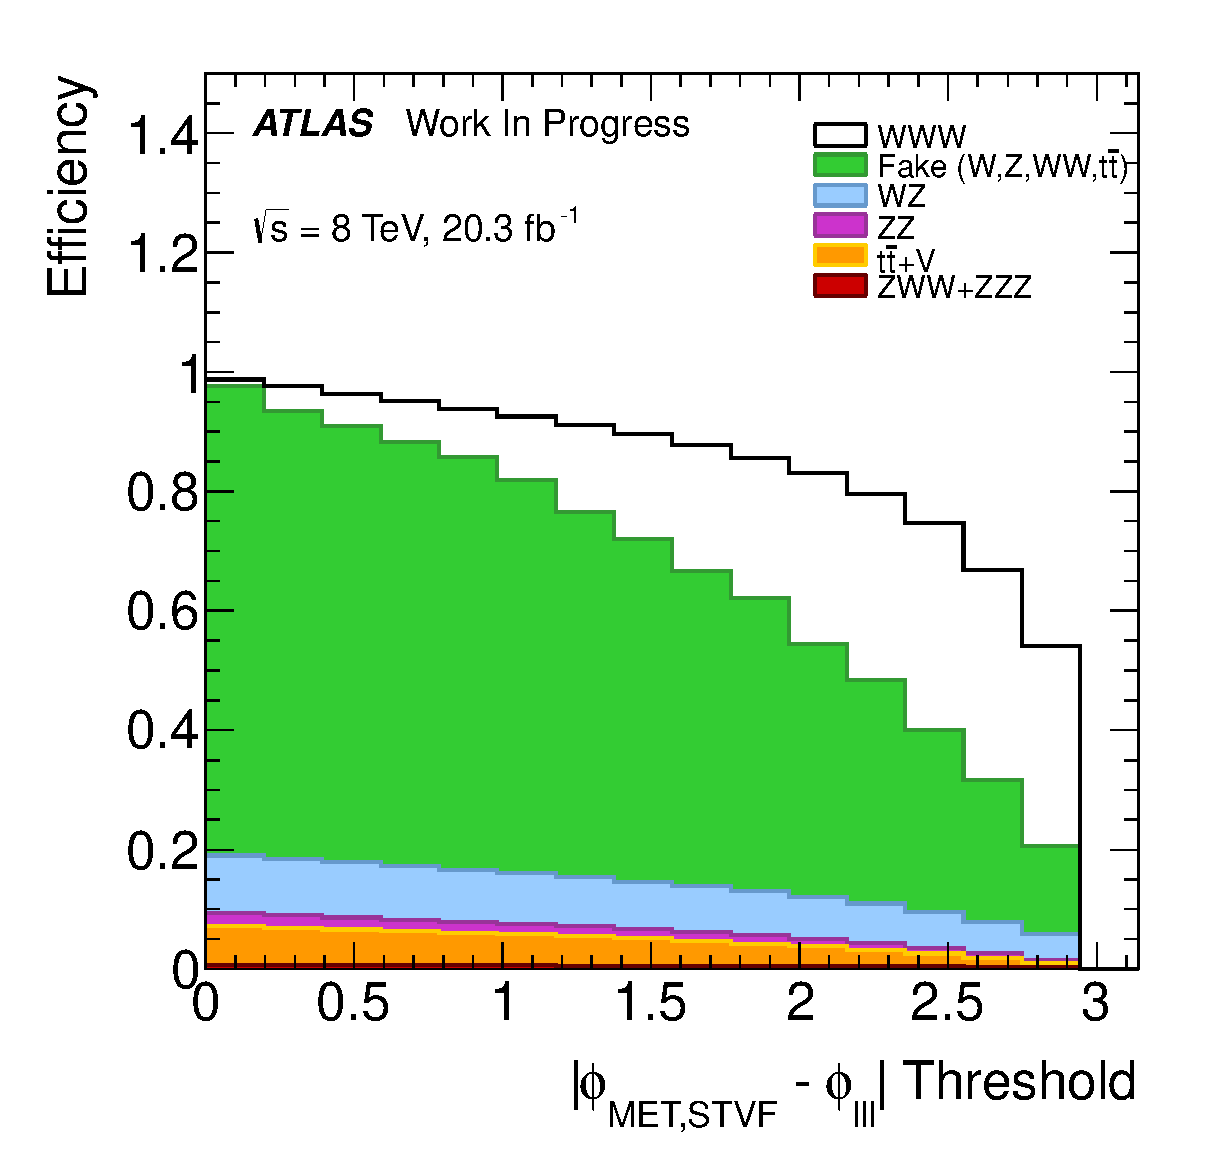
\includegraphics[width=0.45\columnwidth]{figures/optimization/SignalRegionsPreselection_0SFOS_Efficiencies/DeltaPhiMETSTVF123_Abs_Cumulative.eps}
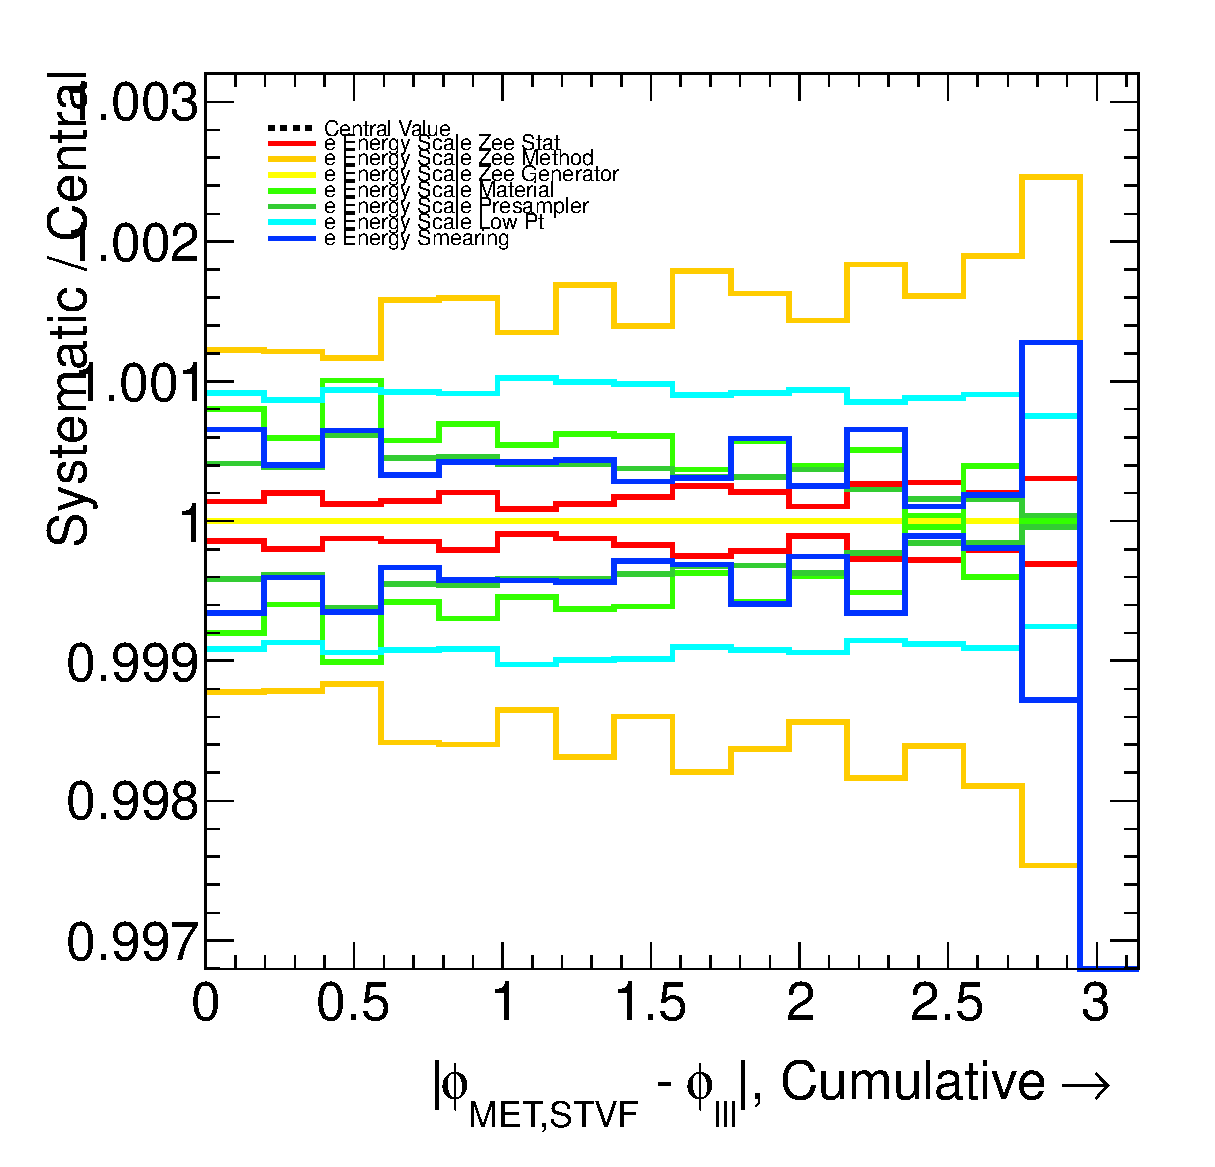
\includegraphics[width=0.45\columnwidth]{figures/optimization/SignalRegions_0p5mmZ0_Preselection_Efficiencies/DeltaPhiMETSTVF123_Abs_Cumulative.eps}
\caption{ Signal and background efficiencies 
for the selection
$|\deltaphi| > X$
as a function of the \deltaphi~selection
threshold, $X$, in both the 0 SFOS (left) and pre-selection (right) regions.  }
\label{fig:deltaphi_eff}
\end{figure}

The efficiencies as a function of the lepton \pt~threshold are shown 
in \fig\ref{fig:pt_eff}. 
The signal efficiency is observed to be slightly flatter
than the background efficiency.
The signal efficiency, however,  still falls fairly 
rapidly as a function of the lepton \pt~threshold. 
Thus, a tighter selection on the lepton \pt~is not preferred
by the optimization. We also considered 
applying different \pt~thresholds to the leptons
based on their \pt~order and other criteria, but
this did not show any increased performance.


\begin{figure}[ht!]
\centering
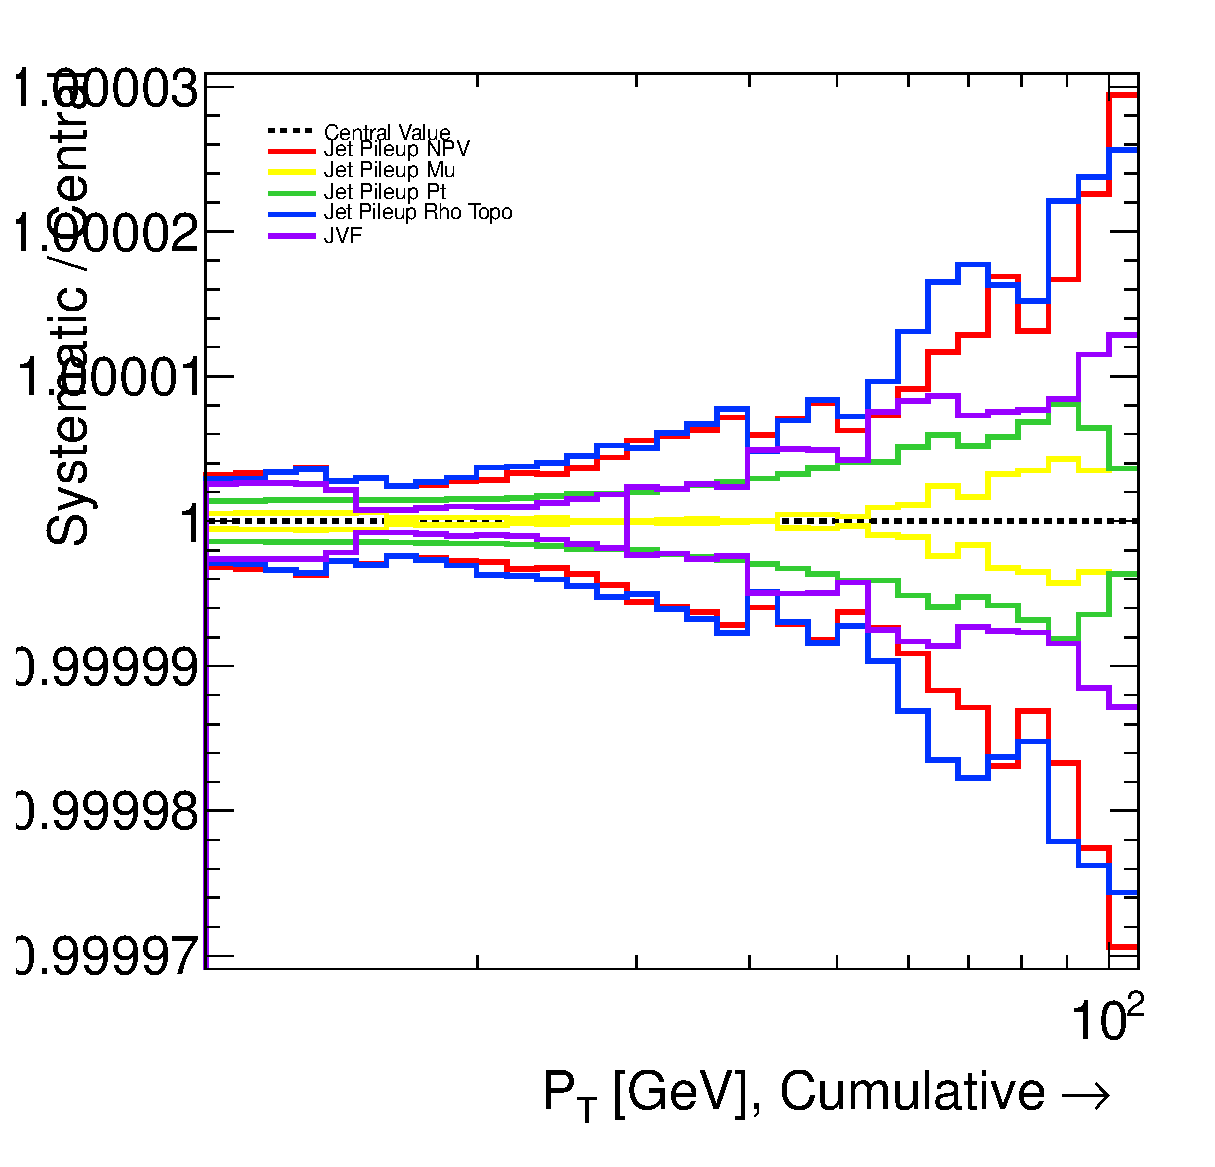
\includegraphics[width=0.45\columnwidth]{figures/optimization/SignalRegionsPreselection_0SFOS_Efficiencies/AllLeptonPt_Cumulative.eps}
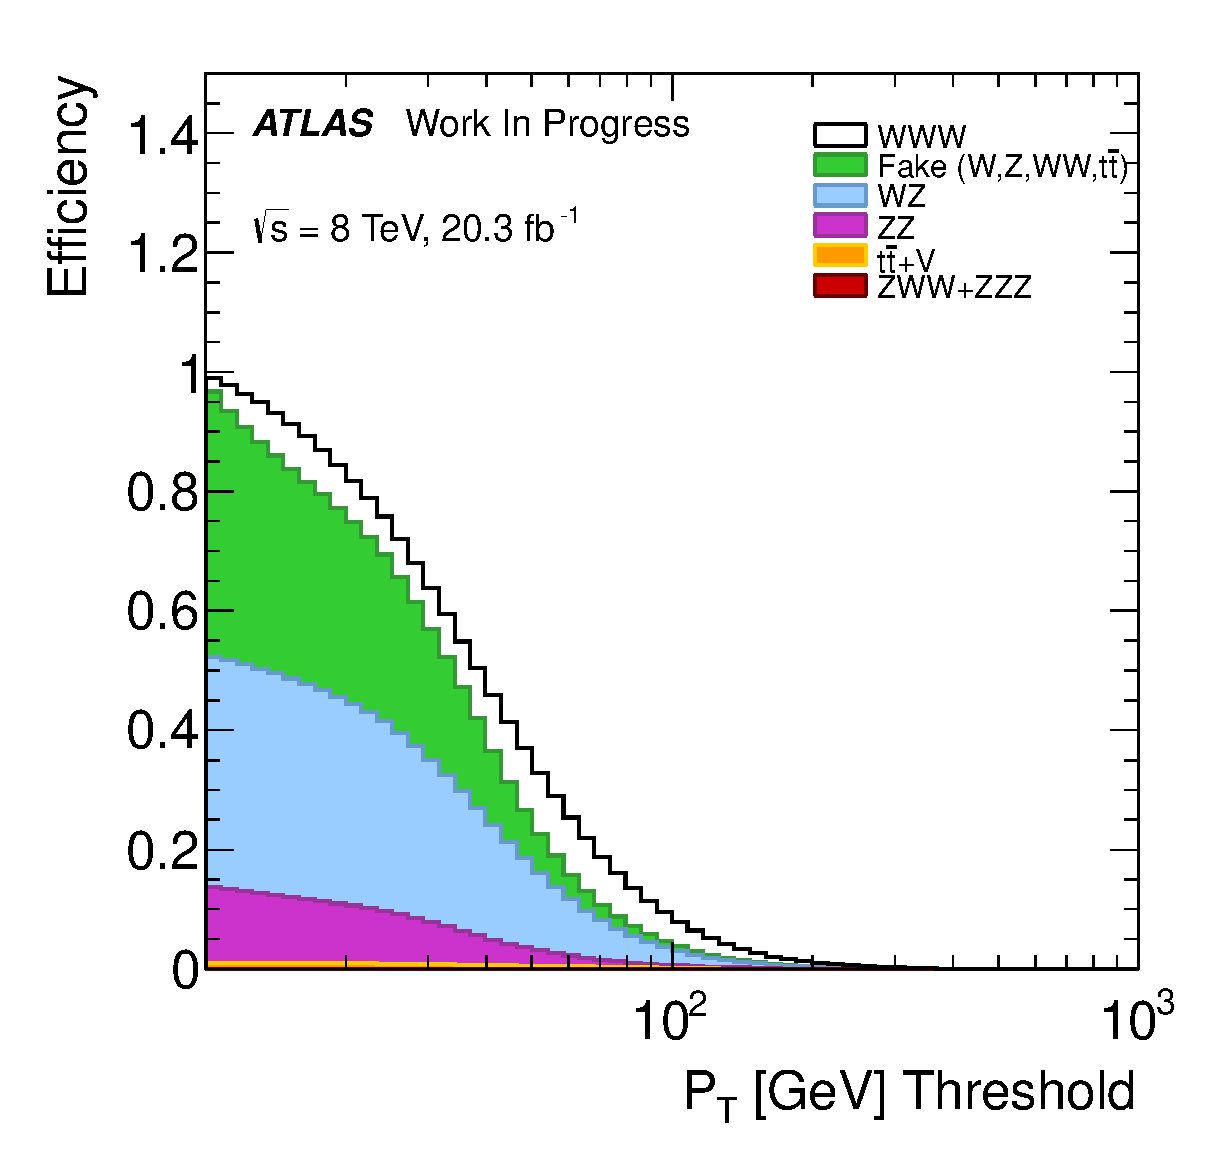
\includegraphics[width=0.45\columnwidth]{figures/optimization/SignalRegions_0p5mmZ0_Preselection_Efficiencies/AllLeptonPt_Cumulative.eps}
\caption{ Signal and background efficiencies 
for the selection
Lepton $\pt > X$
as a function of the \pt~selection
threshold, $X$, in both the 0 SFOS (left) and pre-selection (right) regions.  }
\label{fig:pt_eff}
\end{figure}

Finally, we considered other quantities like the 
transverse mass of the \MET~and three lepton system:
\begin{equation}
m_{T}^{lll} = \sqrt{2p_{T}^{lll}\MET(1-\cos(\Delta\varphi(lll,\MET)))}
\end{equation}
as well as vetoes on additional leptons with lower \pt, and various
di-lepton mass selections.  None of these, however, were preferred
by the optimization.



\FloatBarrier
\section{Event Yields}
\label{sec:event_yield}


\subsection{Event Pre-selection}
\label{sec:preselection_yield}

\begin{figure}[ht!]
\centering
%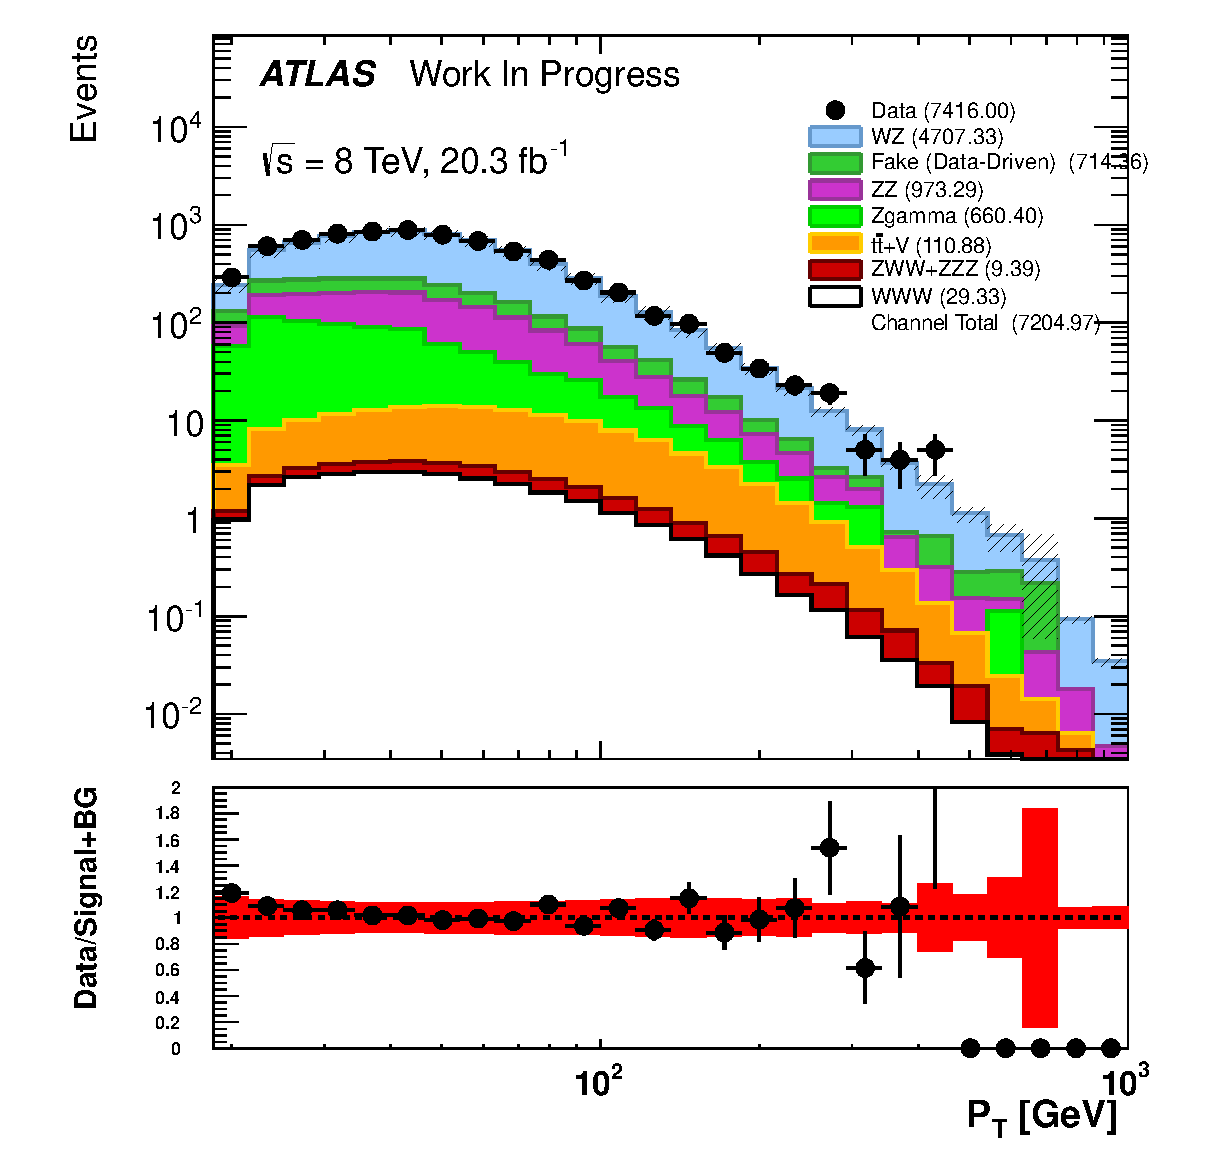
\includegraphics[width=0.3\columnwidth]{figures/appendix_signal_selection/Nov24Update_FakeSys_KFacSys_LogY_NoRebin/output/jobs/MxM/DataFull_Rates_May13_FakeRatesExactly2Loose_MuonMxMBJetGt0_ElBJetGt0SubtractPC_MxM/PreselectionNov23_15_physics/weight_all/eps/AllLeptonPt_histratio.eps}
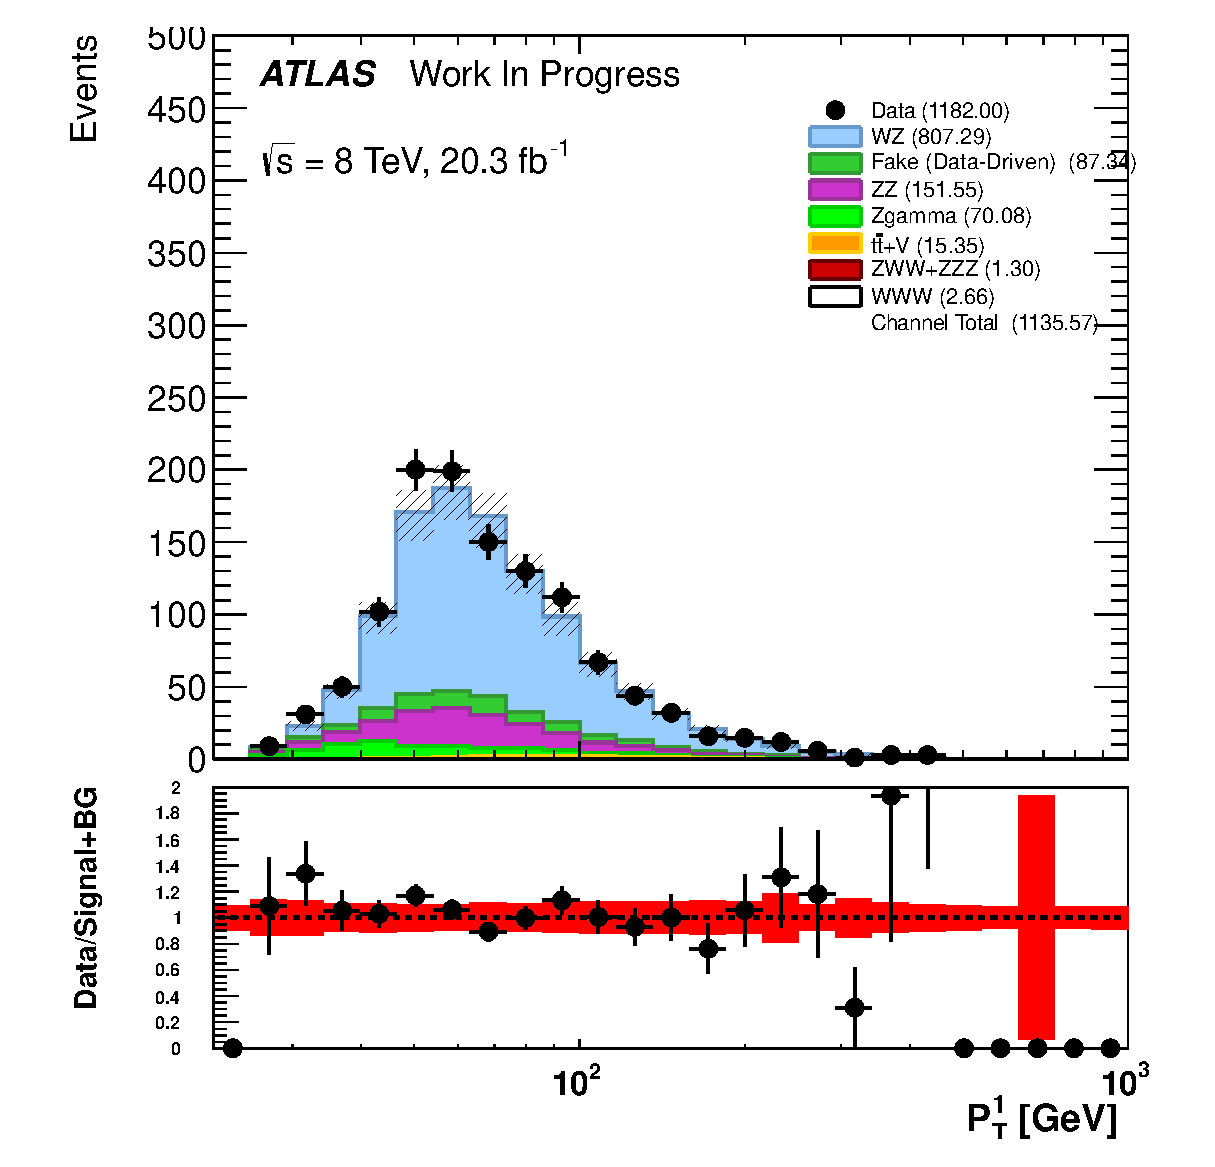
\includegraphics[width=0.3\columnwidth]{figures/appendix_signal_selection/Nov24Update_FakeSys_KFacSys_LogY_NoRebin/output/jobs/MxM/DataFull_Rates_May13_FakeRatesExactly2Loose_MuonMxMBJetGt0_ElBJetGt0SubtractPC_MxM/PreselectionNov23_15_physics/weight_all/eps/LeadingLeptonPt_histratio.eps}
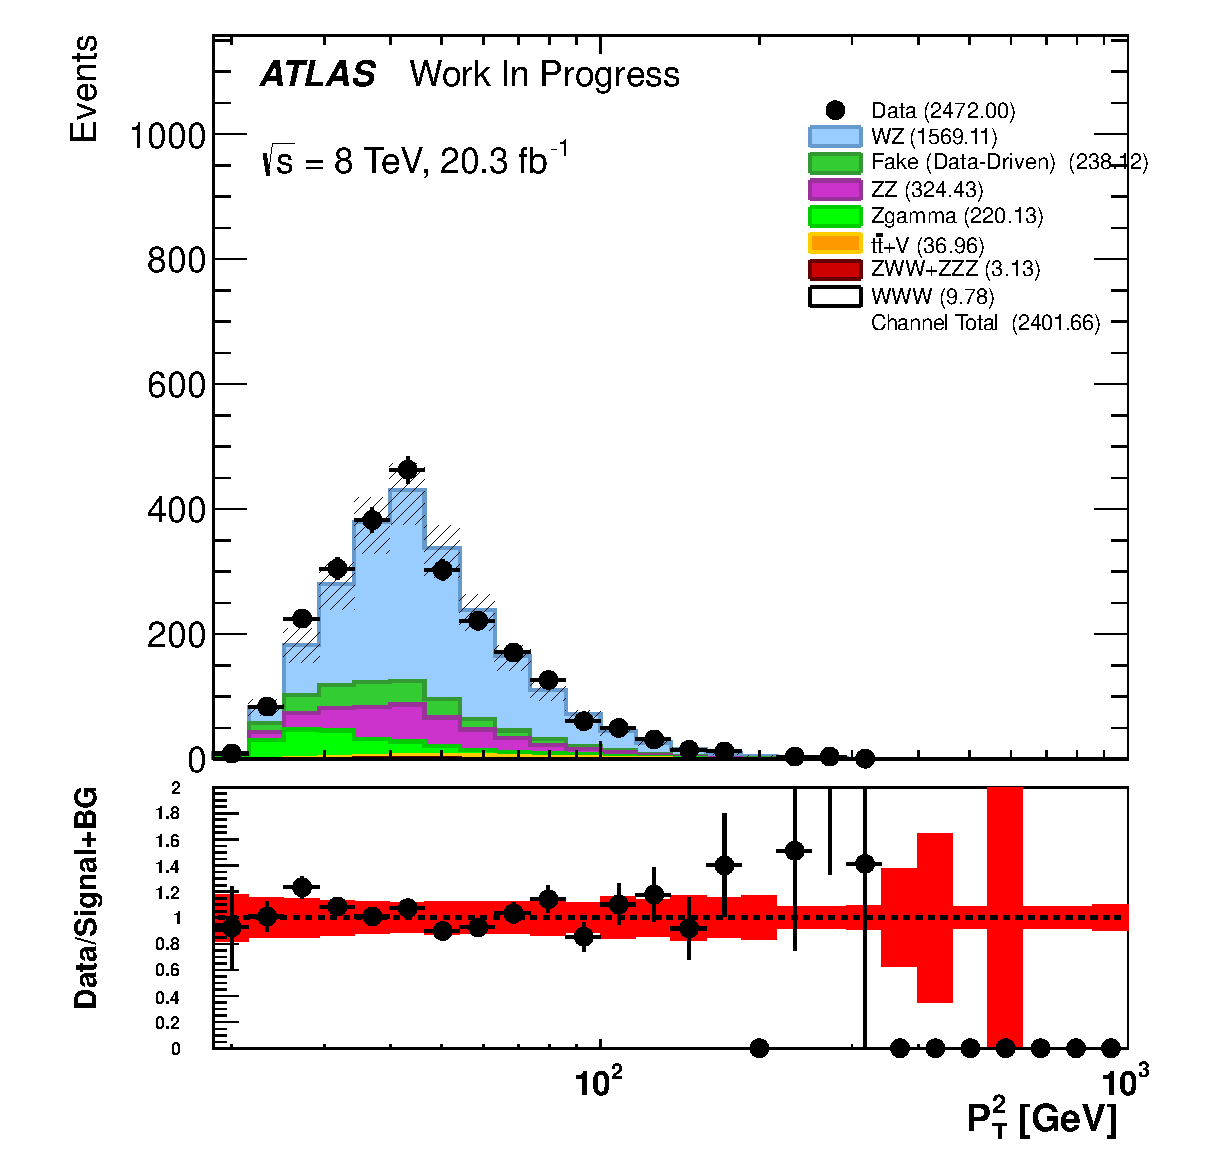
\includegraphics[width=0.3\columnwidth]{figures/appendix_signal_selection/Nov24Update_FakeSys_KFacSys_LogY_NoRebin/output/jobs/MxM/DataFull_Rates_May13_FakeRatesExactly2Loose_MuonMxMBJetGt0_ElBJetGt0SubtractPC_MxM/PreselectionNov23_15_physics/weight_all/eps/SubleadingLeptonPt_histratio.eps}
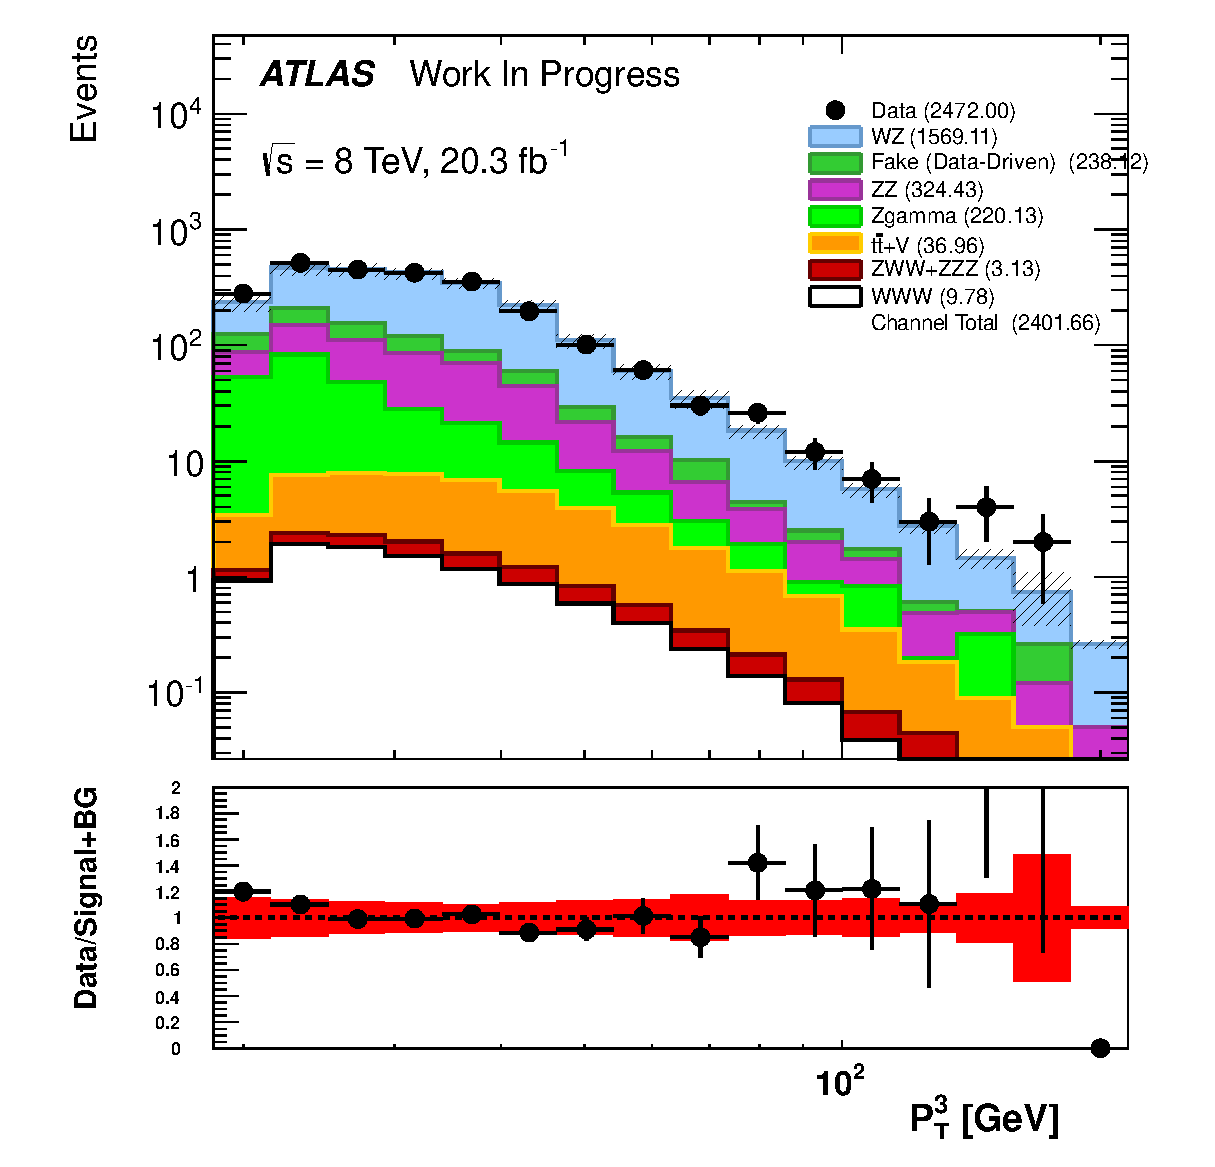
\includegraphics[width=0.3\columnwidth]{figures/appendix_signal_selection/Nov24Update_FakeSys_KFacSys_LogY_NoRebin/output/jobs/MxM/DataFull_Rates_May13_FakeRatesExactly2Loose_MuonMxMBJetGt0_ElBJetGt0SubtractPC_MxM/PreselectionNov23_15_physics/weight_all/eps/MinimumLeptonPt_histratio.eps}
\includegraphics[width=0.3\columnwidth]{figures/appendix_signal_selection/Nov24Update_FakeSys_KFacSys_LogY_NoRebin/output/jobs/MxM/DataFull_Rates_May13_FakeRatesExactly2Loose_MuonMxMBJetGt0_ElBJetGt0SubtractPC_MxM/PreselectionNov23_15_physics/weight_all/eps/MET_Et_histratio.eps}
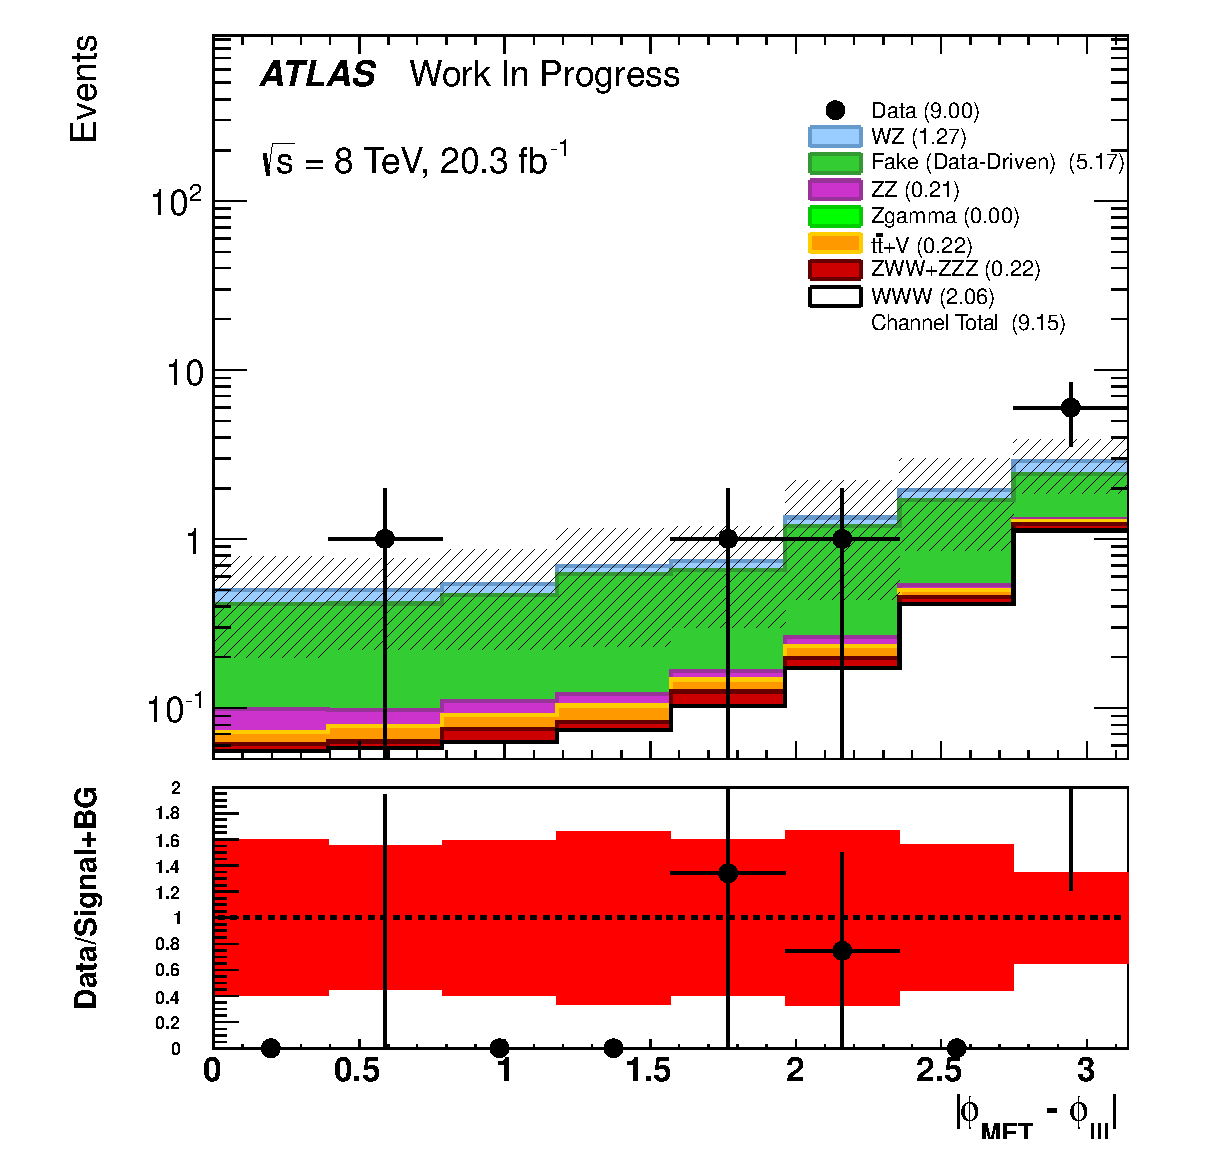
\includegraphics[width=0.3\columnwidth]{figures/appendix_signal_selection/Nov24Update_FakeSys_KFacSys_LogY_NoRebin/output/jobs/MxM/DataFull_Rates_May13_FakeRatesExactly2Loose_MuonMxMBJetGt0_ElBJetGt0SubtractPC_MxM/PreselectionNov23_15_physics/weight_all/eps/DeltaPhiMET123_Abs_histratio.eps}
\includegraphics[width=0.3\columnwidth]{figures/appendix_signal_selection/Nov24Update_FakeSys_KFacSys_LogY_NoRebin/output/jobs/MxM/DataFull_Rates_May13_FakeRatesExactly2Loose_MuonMxMBJetGt0_ElBJetGt0SubtractPC_MxM/PreselectionNov23_15_physics/weight_all/eps/InvariantMassSFOS_histratio.eps}
\includegraphics[width=0.3\columnwidth]{figures/appendix_signal_selection/Nov24Update_FakeSys_KFacSys_LogY_NoRebin/output/jobs/MxM/DataFull_Rates_May13_FakeRatesExactly2Loose_MuonMxMBJetGt0_ElBJetGt0SubtractPC_MxM/PreselectionNov23_15_physics/weight_all/eps/NBTaggedJets_histratio.eps}
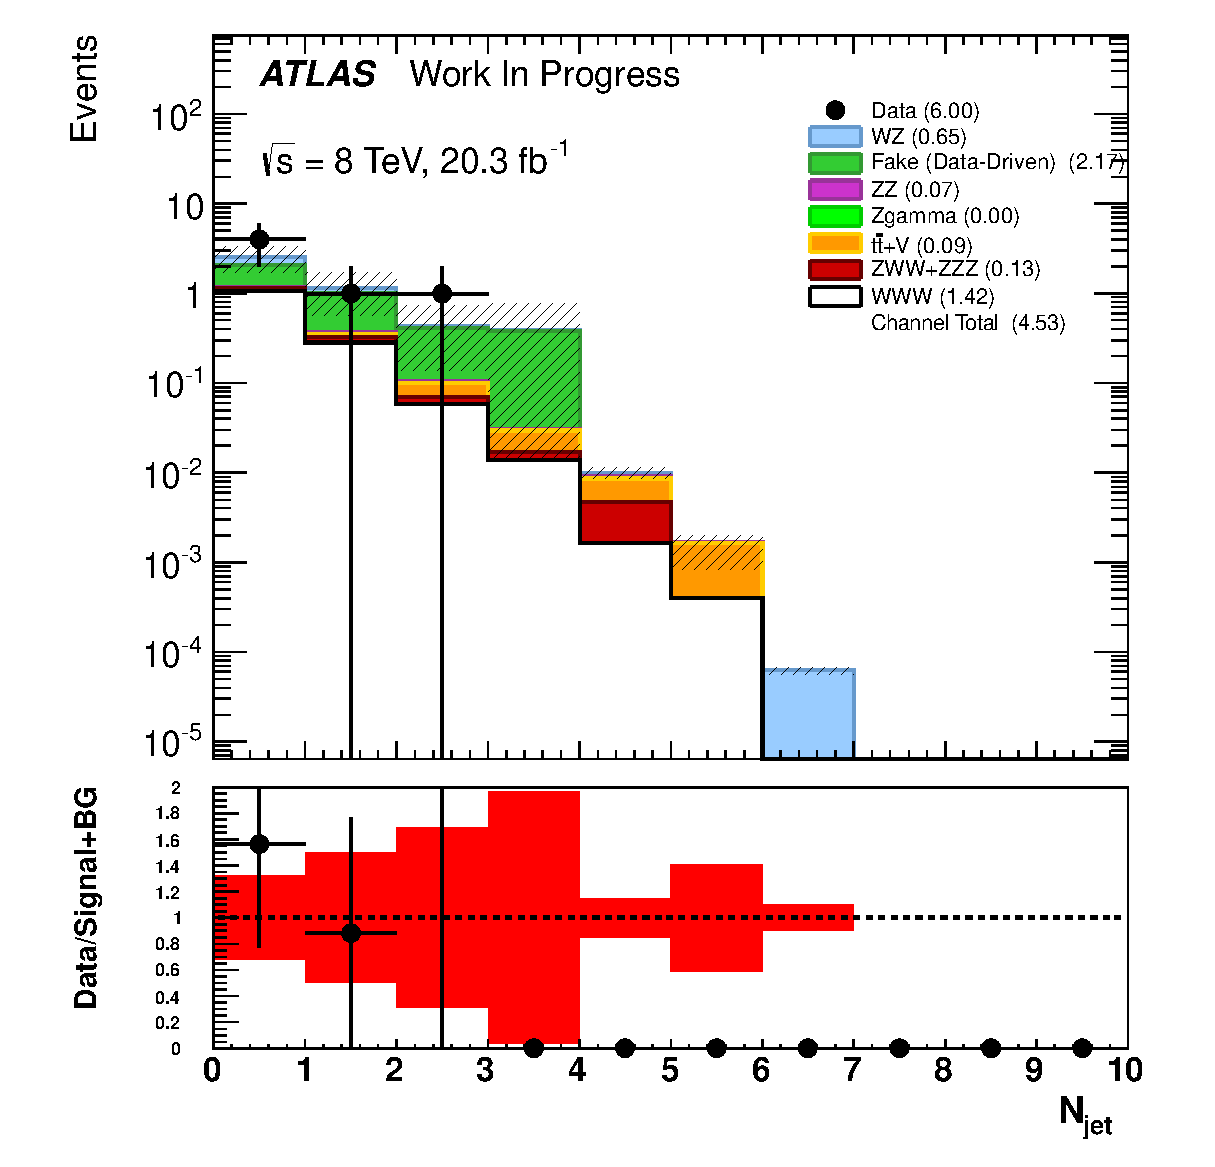
\includegraphics[width=0.3\columnwidth]{figures/appendix_signal_selection/Nov24Update_FakeSys_KFacSys_LogY_NoRebin/output/jobs/MxM/DataFull_Rates_May13_FakeRatesExactly2Loose_MuonMxMBJetGt0_ElBJetGt0SubtractPC_MxM/PreselectionNov23_15_physics/weight_all/eps/NJets_histratio.eps}
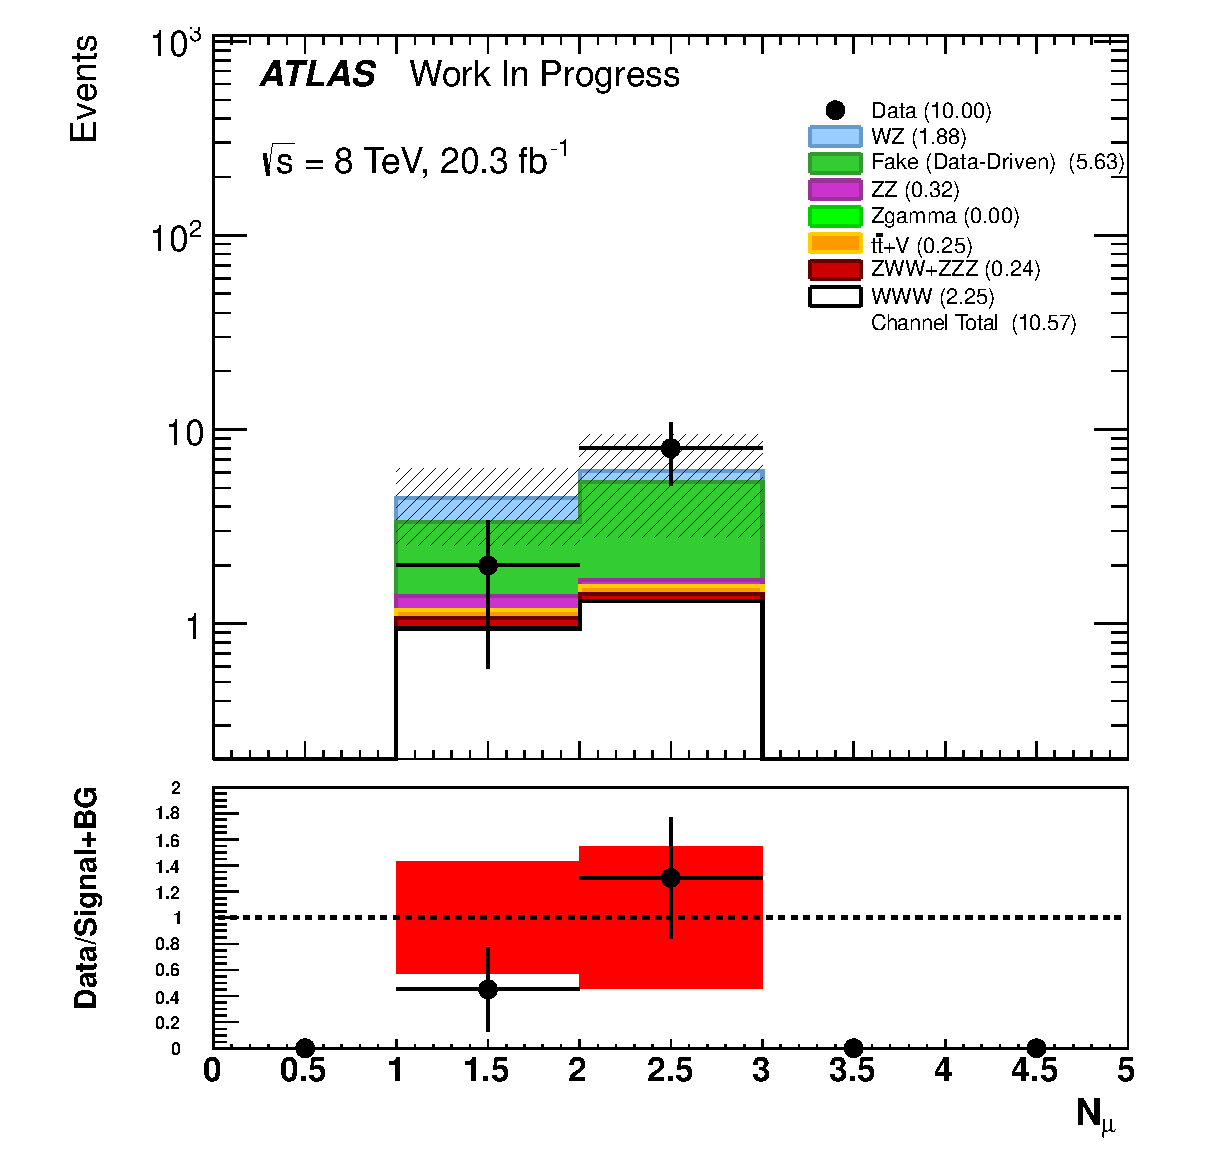
\includegraphics[width=0.3\columnwidth]{figures/appendix_signal_selection/Nov24Update_FakeSys_KFacSys_LogY_NoRebin/output/jobs/MxM/DataFull_Rates_May13_FakeRatesExactly2Loose_MuonMxMBJetGt0_ElBJetGt0SubtractPC_MxM/PreselectionNov23_15_physics/weight_all/eps/NMuons_histratio.eps}
%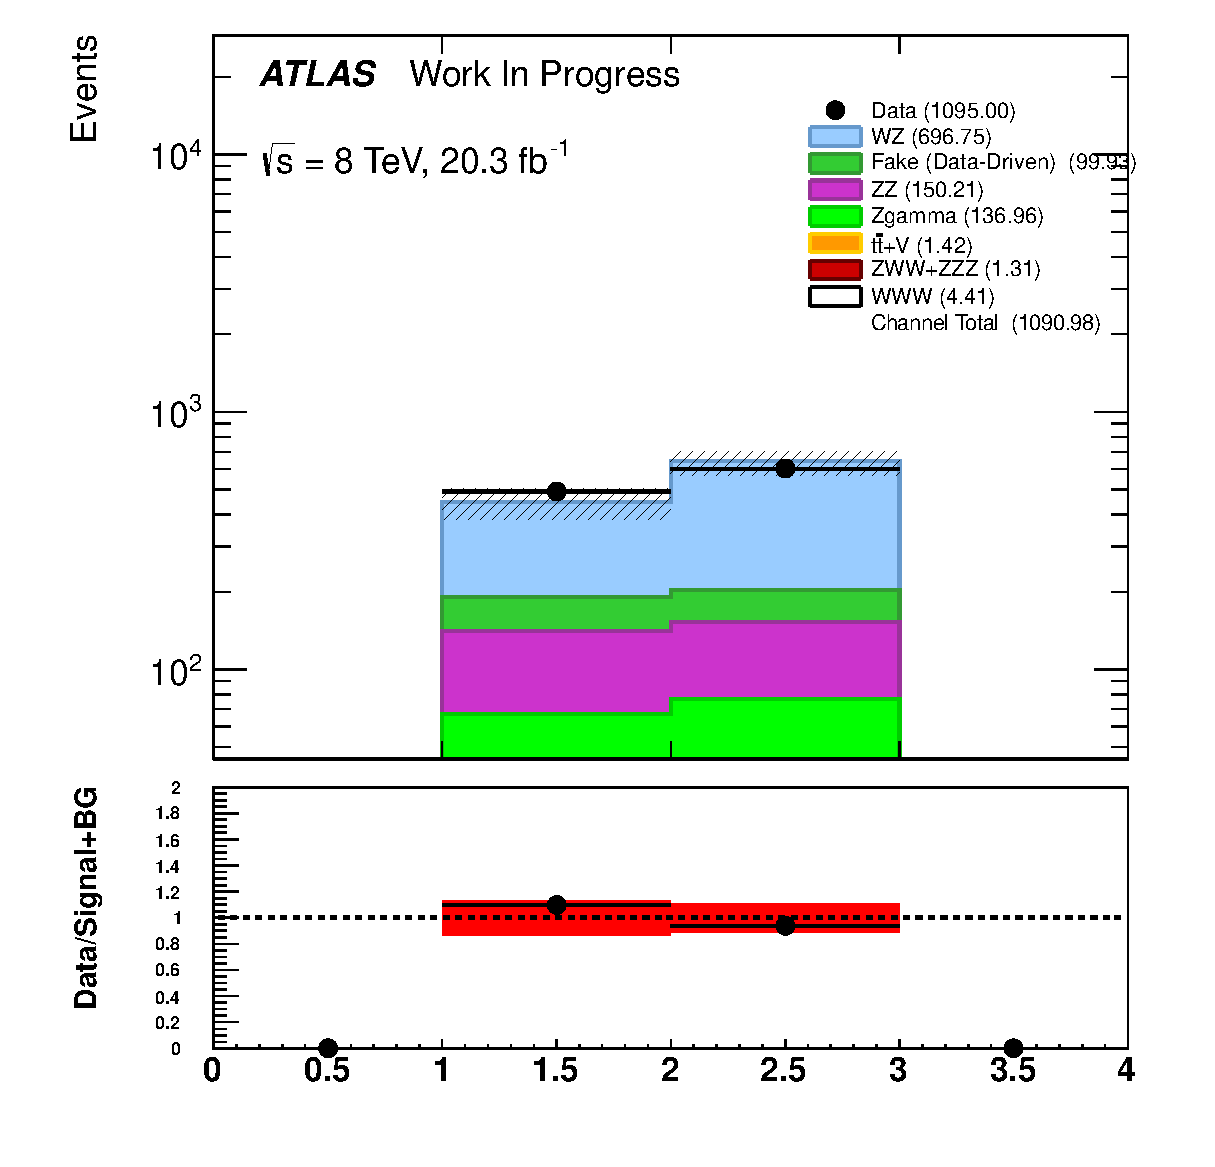
\includegraphics[width=0.3\columnwidth]{figures/appendix_signal_selection/Nov24Update_FakeSys_KFacSys_LogY_NoRebin/output/jobs/MxM/DataFull_Rates_May13_FakeRatesExactly2Loose_MuonMxMBJetGt0_ElBJetGt0SubtractPC_MxM/PreselectionNov23_15_physics/weight_all/eps/TotalCharge_histratio.eps}
\caption{Distributions showing the observed data compared to the background estimate at event pre-selection.}
\label{fig:preselection}
\end{figure}
The signal plus background model 
(described in detail in \sec\ref{sec:bg_estimates})
is compared to data at pre-selection, defined in \sec\ref{sec:preselection},
for a few different kinematic distributions 
in \fig\ref{fig:preselection}. In the upper plot of each distribution,
the colored histograms 
represent the different categories contributing to the signal 
plus background model and 
are split by color based on the category. 
%The colors are...
Hashed bands are shown on the stacked
histograms representing the size of the systematic uncertainties 
on the model, described in \sec\ref{}.
The data is shown in the black points where the 
bars on the points represent the statistical uncertainty on the data.
The lower plot shows the ratio of the data over the model.
In this case, the error bars correspond to the statistical uncertainty
on the ratio due to both the data and the model. The red band
shows the size of the systematic uncertainties with respect to the model.
The model is said to be consistent with the data
if the ratio is consistent with unity after considering statistical
and systematic uncertainties.
The different distributions are chosen primarily because 
of their potential to discriminate between signal and background. 
From top to bottom and left to right,
these distributions are: the leading, subleading, and minimum lepton \pt~(ordered by their \pt),
\MET, \deltaphi, $m_{\textrm{SFOS}}$, \njet, \nbjet, and $N_{\mu}$.
In general, the signal plus background model is observed to be consistent
with the data at the pre-selection, at least for those distributions
considered here.




%\begin{table}[ht!]
%\centering
%\begin{tabular}{|c||c|c|c|c|}
\hline
 & $eee$ & $ee\mu$ & $e\mu\mu$ & $\mu\mu\mu$\\ 
\hline\hline
$WZ$ &  $240.85 \pm 0.67$ &  $339.17 \pm 0.82$ &  $422.07 \pm 0.87$ &  $567.0 \pm 1$\\ 
$ZZ$ &  $60.21 \pm 0.13$ &  $54.1 \pm 0.2$ &  $118.60 \pm 0.31$ &  $91.48 \pm 0.17$\\ 
$Z\gamma$ &  $70.1 \pm 2.7$ &  $0.47 \pm 0.22$ &  $149.4 \pm 3.9$ &  $0.17 \pm 0.12$\\ 
$ZWW+ZZZ$ &  $0.436 \pm 0.019$ &  $0.834 \pm 0.027$ &  $1.00 \pm 0.03$ &  $0.864 \pm 0.028$\\ 
$t\bar{t}+V$ &  $4.854 \pm 0.044$ &  $9.549 \pm 0.064$ &  $12.047 \pm 0.072$ &  $10.510 \pm 0.066$\\ 
Fake (data-driven) &  $45.1 \pm 2.2$ &  $37.8 \pm 1.6$ &  $112.7 \pm 2.8$ &  $42.5 \pm 1.2$\\ 
$WWW$ &  $0.770 \pm 0.011$ &  $3.023 \pm 0.023$ &  $3.970 \pm 0.026$ &  $1.843 \pm 0.018$\\ 
\hline
Expected Background &  $421.6 \pm 3.5$ &  $441.9 \pm 1.8$ &  $815.8 \pm 4.9$ &  $712.5 \pm 1.6$\\ 
Expected Signal + Background &  $422.4 \pm 3.5$ &  $444.9 \pm 1.8$ &  $819.8 \pm 4.9$ &  $714.4 \pm 1.6$\\ 
\hline
Observed Data &  $426 \pm 21$ &  $468 \pm 22$ &  $821 \pm 29$ &  $757 \pm 28$\\ 
\hline
\end{tabular}

%\caption{Expected and observed event yields binned by lepton flavor combination at event pre-selection.
%Only statistical uncertainties are shown.
%}
%\label{tab:preselection}
%\end{table}



\begin{figure}[ht!]
\centering
\includegraphics[width=0.5\columnwidth]{figures/SFOSPreselection.png}
\caption{Yields at event pre-selection in the 0, 1 and 2 SFOS regions.  
The most important systematic uncertainties 
(discussed in section~\ref{sec:systematics}) are shown, 
namely from the fake estimates and the uncertainties on the WZ and ZZ k-factors.}
\label{fig:preselection_nsfos}
\end{figure}

Upon splitting the pre-selection region based on the number of SFOS
pairs, we end up with signal and background predictions like in 
\fig\ref{fig:preselection_nsfos}, where we can see differences
in the branching fraction for the signal to each of the three signal regions.
In the 0 and 2 SFOS regions, roughly 2.5 signal events are predicted
whereas closer to 5 signal events are predicted in the 1 SFOS region. 
Totaling about 10 signal events predicted at the pre-selection stage.
Shifting to looking at the background, perhaps the most striking 
feature of this plot is the 
clear difference in background yield and background composition
between the 0 SFOS region and the 1 and 2 SFOS regions.
More than 1000 background events are predicted in both the 1 and
the 2 SFOS regions, while only about 30 background events are
predicted in the 0 SFOS region.
Apparently then, the advantage of splitting the signal region based on this
classification comes when looking at the background, specifically the
electroweak $WZ$ and $ZZ$ backgrounds where SFOS lepton pairs may be
produced from the decay of the $Z$ boson(s). Consider only the case
where the $WZ$ and $ZZ$ decay to either $e$ or $\mu$.  The $WZ$ production
process is thus characterized by 3 leptons with at least 1 SFOS lepton pair
which comes from the $Z$. If all three leptons from the $WZ$ decay have been
reconstructed, then there is a 50~\% chance the third lepton 
will also be able to form a SFOS pair with one of the leptons from the $Z$ decay.
Thus, the WZ background will split evenly between the 1 and 2 SFOS classification.
Something similar occurs for the ZZ background except that the fourth lepton 
in the decay must be lost (usually due to possessing a low $\pt$).
The large cross-section for theses processes means that
they become the dominant backgrounds in the 1 and 2 SFOS regions.  
The 0 SFOS signal region is mostly spared from contamination  by 
these large processes but still
includes both the $WZ$ and $ZZ$ processes as background due to the
non-negligible (albeit small) effect of mis-measurement of the lepton
charge, see section~\ref{sec:chargeMisID}.  The 0 SFOS signal region
is thus unique in having a small background which is almost entirely
reducible and dominated instead by events where a jet is mis-measured
as or overlaps with a lepton, called the fake lepton background, along
with the aforementioned sub-dominant effect of lepton charge 
mis-identification described in Section~\ref{sec:chargeMisID}.  

\subsection{Optimization}
\label{sec:optimization}
From the above discussion, one can clearly see that it is
advantageous to split these signal regions so that the dominant
backgrounds in each region may be targeted individually.  Furthermore,
note that even though the 1 SFOS region contains more of the signal than the
0 and 2 SFOS regions, it is the 0 SFOS region which is most likely to
have the best sensitivity due to the smaller background contribution.
In \sec\ref{sec:signal_regions} it was already shown
that a selection was chosen based on an optimization procedure
designed to further reduce the background with respect to the 
signal region. 

The optimization takes as input a multi-dimensional 
space where each dimension is the selection threshold
for one of the quantities listed in \tab\ref{tab:signal_selection}, 
plus some others.
The range of the multi-dimensional space 
is restricted so that the 
predicted signal remains finite i.e. non-zero.
At an individual point in this space, the optimization computes
the expected signal and background events after the selection
along with the size of statistical uncertainties
and systematic uncertainties on the model. 
These are then used as input to the measurement extraction framework
described in \sec\ref{sec:measurement} to determine the width of the precision
on the final measurement. 
This width is used as the metric to minimize in the optimization.
By considering a metric like this, we are optimizing directly
the quantity of interest to the final measurement, and taking
into account not just the individual predictions, but also their
uncertainties. This is important because it can more stringently
remove backgrounds that have large uncertainties.

We choose to treat the sample space as being discrete as opposed
to continuous. For some dimensions of the space, such as 
the threshold on \njet, this is manifestly true, as there 
can only be an integer number of observed jets. 
For other dimensions, such as the threshold on the lepton
\pt, these quantities are real valued and thus continuous.
%looking at \fig\ref{fig:optimization_efficiencies_preselection} 
%and \fig\ref{fig:optimization_efficiencies_0sfos}, 
%the shape of the efficiencies tend to change relatively slowly from bin to bin 
It should be acceptable to only sample 
discretely, however,  as long as they can capture the shape information of 
the efficiencies. % as they do above. 
Furthermore, 
this acknowledges the finite  experimental resolution of these 
quantities. For example,
the difference between $\pt > 20~\GeV$ and $\pt > 20.5~\GeV$
should not be taken too seriously because of the effects of limited
track and energy resolution used to derive the muon and electron \pt.
%expand on this? what would be the typical electron and muon resolution here?
Treating the sample space as discrete means that the optimization
function is not smooth and so cannot readily take into account
derivative information to be used for instance 
in some sophisticated minimization algorithm.
Fortunately, the number of points in the sample space after discretizing, 
though large, is small enough that it can be evaluated in its entirety
using a brute force approach. Thus, we choose to evaluate the 
optimization in the restricted and discretized sample space in order
to find an optimal choice for the selection.

%I should redo the optimization for the specific bin sizes and list them

The shape of the optimization can be seen in \fig\ref{fig:optimization}.
\emph{Figures need to be reproduced. Elaborate...} 


\begin{figure}[ht!]
\centering

\includegraphics[width=0.3\columnwidth]{figures/placeholder.eps}

\includegraphics[width=0.3\columnwidth]{figures/placeholder.eps}

\includegraphics[width=0.3\columnwidth]{figures/placeholder.eps}
\caption{Signal Yield vs Measurement Uncertainty for optimized points 
in the 0 SFOS (left), 1 SFOS (middle), and 2 SFOS (right) signal regions.}
\label{fig:optimization}
\end{figure}


The final selection is presented in \tab\ref{tab:signal_selection}.
Details of the specific cut thresholds that are chosen can be understood
by looking closer at some of the quantities used as input to 
the optimization. For instance, it is observed that
different \MET~and \z-veto thresholds are chosen for the 1 and 2 SFOS
regions. This can be understood to come from a correlation between
these two quantities due to their ability to isolate the $Z\gamma$
background.
The $Z\gamma$ background shows up in the low-shoulder of the \z-peak
in the $m_{\textrm{SFOS}}$ distribution and at low MET. This can be
seen both for the 1 and 2 SFOS regions in \fig\ref{fig:met_zwindow_optimization}.
As a result, the $Z\gamma$ background can be removed either by tuning 
the \z-mass window used in the veto above, or by removing events with low \met.
Thus, the optimization shows that there is some correlation 
between the \z-veto window and the \met~selection threshold. 
In the 1 SFOS region, there is a larger 
contribution from $Z\gamma$ processes than in the 2 SFOS
region.  This process mostly shows up in the low shoulder 
of the \z~ peak. The optimization
prefers removing this $Z\gamma$ contribution by setting an 
asymmetric \z-window in the 1 SFOS
region, with the boundaries being 35~GeV below the \z-pole 
and 20~GeV above and then keeping the \MET~cut a little loose, with a 
threshold of $\MET > 45$~GeV.  In the 2 SFOS region, however,
the $Z\gamma$ contribution is not as prominent and the 
optimization happens to prefer a symmetric
window of $\pm20$~GeV around the \z-pole.  
The looser \z-veto then allows for a tighter
missing $E_{T}$ cut with a threshold of $\MET > 55$~GeV. 

\begin{figure}[ht!]
\centering
\includegraphics[width=0.4\columnwidth]{figures/appendix_signal_selection/Nov24Update_FakeSys_KFacSys_LogY_NoRebin/output/jobs/MxM/DataFull_Rates_May13_FakeRatesExactly2Loose_MuonMxMBJetGt0_ElBJetGt0SubtractPC_MxM/PreselectionNov23_15_1SFOS_ChargeAbs1_BVeto85_physics/weight_all/png/MET_Et_histratio.png}
\includegraphics[width=0.4\columnwidth]{figures/appendix_signal_selection/Nov24Update_FakeSys_KFacSys_LogY_NoRebin/output/jobs/MxM/DataFull_Rates_May13_FakeRatesExactly2Loose_MuonMxMBJetGt0_ElBJetGt0SubtractPC_MxM/PreselectionNov23_15_1SFOS_ChargeAbs1_BVeto85_physics/weight_all/png/InvariantMassSFOS_histratio.png}
\includegraphics[width=0.4\columnwidth]{figures/appendix_signal_selection/Nov24Update_FakeSys_KFacSys_LogY_NoRebin/output/jobs/MxM/DataFull_Rates_May13_FakeRatesExactly2Loose_MuonMxMBJetGt0_ElBJetGt0SubtractPC_MxM/PreselectionNov23_15_2SFOS_ChargeAbs1_BVeto85_physics/weight_all/png/MET_Et_histratio.png}
\includegraphics[width=0.4\columnwidth]{figures/appendix_signal_selection/Nov24Update_FakeSys_KFacSys_LogY_NoRebin/output/jobs/MxM/DataFull_Rates_May13_FakeRatesExactly2Loose_MuonMxMBJetGt0_ElBJetGt0SubtractPC_MxM/PreselectionNov23_15_2SFOS_ChargeAbs1_BVeto85_physics/weight_all/png/InvariantMassSFOS_histratio.png}
\caption{Plots of the \MET (left) and $m_{\textrm{SFOS}}$ (right) distributions 
in the 1 SFOS (top) and 2 SFOS (bottom) regions after pre-selection
plus the \bee-veto requirement.}
\label{fig:met_zwindow_optimization}
\end{figure}

The absence of any cut on the \MET~distribution in the 0 SFOS
region can be better understood by looking at the 
the efficiency for selection between 
the signal and the background as a function of the \MET~selection threshold.
This is shown in \fig\ref{fig:met_eff} both after pre-selection
and in the 0 SFOS region.
Clearly, the signal efficiency closely follows the background efficiency
in the 0 SFOS region. Thus, there is no change in the
signal-to-background ratio when cutting on the \MET~distribution
in the 0 SFOS region and thus no improvement in the sensitivity.
On the other hand, there are large shape differences 
between the signal
and background efficiencies at pre-selection, with the 
signal efficiency remaining flatter at low values of the \MET~
threshold. So, from this one would expect a selection
on the \MET~threshold to be useful in the 1 and 2 SFOS
regions which have a similar background composition. 
Indeed, this is what we observe.


\begin{figure}[ht!]
\centering
\includegraphics[width=0.45\columnwidth]{figures/optimization/SignalRegionsPreselection_0SFOS_Efficiencies/MET_Et_STVF_Cumulative.eps}
\includegraphics[width=0.45\columnwidth]{figures/optimization/SignalRegions_0p5mmZ0_Preselection_Efficiencies/MET_Et_STVF_Cumulative.eps}
\caption{ Signal and background efficiencies for the 
selection $\MET > X$ as a function of the \MET~selection
threshold, $X$,  in both the 0 SFOS (left) and pre-selection (right) regions.  }
\label{fig:met_eff}
\end{figure}

The threshold for the jet multiplicity cut 
of $\njet\leq 1$ applied in all signal regions
is also determined from the optimization. One might expect
that a different value for the threshold, such as a complete
veto on the presence of jets, would perform better. 
Indeed, looking at the efficiency for selection on the jet multiplicity
in \fig\ref{fig:njet_eff} does show a much stronger background
rejection when applying a veto in both the pre-selection region
and especially in the 0 SFOS region where there is a larger
contribution from fakes due to hadronic activity.
The signal rejection, however,  of about 40\% observed in both
regions, is prohibitive. Loosening the selection to the nominal
threshold of $\njet \leq 1$ instead preserves 90\% of the signal, 
which is quite precious.  We are still able to remove 
much of the fake background in the 0 SFOS region by vetoing
events with \bee-tagged jets as can be seen in \fig\ref{fig:nbjet_eff}.
%any mention of different operating points
It is possible that using a \bee-tagging operating point
with an even higher \bee-tagging efficiency would further 
improve the sensitivity in the 0 SFOS region.  
The nominal operating point used here, however,  is the highest 
efficiency operating point supported by ATLAS.
Clearly, there is no advantage gained from using a looser operating point
as this would only cut less on the background without having an impact
on the signal.



\begin{figure}[ht!]
\centering
\includegraphics[width=0.45\columnwidth]{figures/optimization/SignalRegionsPreselection_0SFOS_Efficiencies/NJets_LeftCumulative.eps}
\includegraphics[width=0.45\columnwidth]{figures/optimization/SignalRegions_0p5mmZ0_Preselection_Efficiencies/NJets_LeftCumulative.eps}
\caption{ Signal and background efficiencies for the selection
$\njet \leq X$ as a function of the \njet~selection
threshold, $X$, in both the 0 SFOS (left) and pre-selection (right) regions.  }
\label{fig:njet_eff}
\end{figure}

\begin{figure}[ht!]
\centering
\includegraphics[width=0.45\columnwidth]{figures/optimization/SignalRegionsPreselection_0SFOS_Efficiencies/NBTaggedJets_LeftCumulative.eps}
\includegraphics[width=0.45\columnwidth]{figures/optimization/SignalRegions_0p5mmZ0_Preselection_Efficiencies/NBTaggedJets_LeftCumulative.eps}
\caption{ Signal and background efficiencies 
for the selection
$\nbjet \leq X$
as a function of the \nbjet~selection
threshold, $X$, in both the 0 SFOS (left) and pre-selection (right) regions.  }
\label{fig:nbjet_eff}
\end{figure}


The \deltaphi~distribution for the signal is observed to be more back-to-back
(i.e. closer to $\pi$)
than that for the background. This is especially true in the 0 SFOS
region, as can be seen from the efficiencies plotted 
as a function of the \deltaphi~
selection threshold shown in \fig\ref{fig:deltaphi_eff}.
The selection efficiency for the signal is relatively flat for
most of the range up to about 
a threshold of $|\deltaphi|>2.5$ in both the pre-selection and 0 SFOS
regions.  At this threshold the signal selection efficiency 
is about 80\%.  The optimization prefers a selection
around this range for all signal regions.
The optimization also considered selecting on alternative
definitions of $\Delta\phi$ that only considered one of the three
leptons but this was observed to not offer as strong of a separation
between the signal and background. %figure?

\begin{figure}[ht!]
\centering
\includegraphics[width=0.45\columnwidth]{figures/optimization/SignalRegionsPreselection_0SFOS_Efficiencies/DeltaPhiMETSTVF123_Abs_Cumulative.eps}
\includegraphics[width=0.45\columnwidth]{figures/optimization/SignalRegions_0p5mmZ0_Preselection_Efficiencies/DeltaPhiMETSTVF123_Abs_Cumulative.eps}
\caption{ Signal and background efficiencies 
for the selection
$|\deltaphi| > X$
as a function of the \deltaphi~selection
threshold, $X$, in both the 0 SFOS (left) and pre-selection (right) regions.  }
\label{fig:deltaphi_eff}
\end{figure}

The efficiencies as a function of the lepton \pt~threshold are shown 
in \fig\ref{fig:pt_eff}. 
The signal efficiency is observed to be slightly flatter
than the background efficiency.
The signal efficiency, however,  still falls fairly 
rapidly as a function of the lepton \pt~threshold. 
Thus, a tighter selection on the lepton \pt~is not preferred
by the optimization. We also considered 
applying different \pt~thresholds to the leptons
based on their \pt~order and other criteria, but
this did not show any increased performance.


\begin{figure}[ht!]
\centering
\includegraphics[width=0.45\columnwidth]{figures/optimization/SignalRegionsPreselection_0SFOS_Efficiencies/AllLeptonPt_Cumulative.eps}
\includegraphics[width=0.45\columnwidth]{figures/optimization/SignalRegions_0p5mmZ0_Preselection_Efficiencies/AllLeptonPt_Cumulative.eps}
\caption{ Signal and background efficiencies 
for the selection
Lepton $\pt > X$
as a function of the \pt~selection
threshold, $X$, in both the 0 SFOS (left) and pre-selection (right) regions.  }
\label{fig:pt_eff}
\end{figure}

Finally, we considered other quantities like the 
transverse mass of the \MET~and three lepton system:
\begin{equation}
m_{T}^{lll} = \sqrt{2p_{T}^{lll}\MET(1-\cos(\Delta\varphi(lll,\MET)))}
\end{equation}
as well as vetoes on additional leptons with lower \pt, and various
di-lepton mass selections.  None of these, however, were preferred
by the optimization.




\subsubsection{Signal Region Yields}
\label{sec:signal_yield}



The selection used in the final signal regions is determined as described in Section~\ref{sec:signal_regions} and is summarized in Table~\ref{tab:signal_selection}. Kinematic distributions are shown for the distribution
that is cut on just before the cut is applied
for each stage of the selection in Figures~\ref{fig:0sfos}, \ref{fig:1sfos}, and \ref{fig:2sfos} for
the 0, 1, and 2 SFOS regions, respectively.
Cut-flows showing the weighted cut-flows at each stage of the signal selection are shown for the 0, 1, and 2 SFOS regions
in Tables ~\ref{tab:cutflow_weighted_0sfos}, ~\ref{tab:cutflow_weighted_1sfos}, ~\ref{tab:cutflow_weighted_2sfos}.
Unweighted cut-flows are shown in appendix~\ref{sec:app_signal_selection}.

%Tables summarizing the event yields after the final
%selection and binned by the lepton flavor combinations are shown in Tables \ref{tab:0sfos}, \ref{tab:1sfos}, and \ref{tab:2sfos}.




\subsubsection{0 SFOS Signal Region}

The cut-flows for the selection in the 0 SFOS region are shown in Table~\ref{tab:cutflow_weighted_0sfos}
while the distributions at each stage of the selection are shown in Figure~\ref{fig:0sfos}.
This is the most sensitive channel with an expected signal to background ratio of 56\%.
The data is observed to agree with the expectation within statistical uncertainties. The background
is ultimately dominated by fake background contributions, which themselves have a large systematic uncertainty
that is similar in size to the statistical uncertainty. This is described in more detail in section~\ref{sec:systematics}.
The Poisson probability of observing 5 events with 3.67 events expected from the signal plus background prediction is 14.1\%.


\begin{table}[ht!]
\centering
\small
\begin{tabular}{l||c|c||c|c||c|c}
\hline
 &                 \multicolumn{2}{c||}{Signal}            &  \multicolumn{2}{c||}{Background} &  \multicolumn{2}{c}{Data} \\
  & Yield & Eff. & Yield & Eff. & Yield & Eff.\\
  \hline\hline
  %1. Pre-selection &  $9.78$ & --- &  $2388.48$ & --- & $2472$ &  --- \\ 
  %\hline
  0 SFOS &  $2.31$ &  --- &  $21.36$ &  --- & $30$ &  ---\\ 
  \hline
  Charge Sum $= \pm 1$ &  $2.30$ &  $1.00$ &  $19.55$ &  $0.92$ & $27$ &  $0.90$\\ 
  \hline
  $N_{\mathrm{b-jet}} = 0$ &  $2.29$ &  $0.99$ &  $8.59$ &  $0.44$ & $10$ &  $0.37$\\ 
  \hline
  $m_{SF} > 20$ GeV &  $2.25$ &  $0.98$ &  $8.32$ &  $0.97$ & $10$ &  $1.00$\\ 
  \hline
  $|m_{ee} - m_{Z}| > 15$ GeV &  $2.06$ &  $0.91$ &  $7.09$ &  $0.85$ & $9$ &  $0.90$\\ 
  \hline
  $|\Delta\phi(3l,E_{T}^{Miss})| > 2.5$ &  $1.41$ &  $0.69$ &  $2.51$ &  $0.35$ & $6$ &  $0.67$\\ 
  \hline
  $N_{\mathrm{Jet}} \leq 1$ &  $1.34$ &  $0.95$ &  $2.35$ &  $0.94$ & $5$ &  $0.83$\\ 
  \hline
  \end{tabular}


\caption{Cut-flows showing the event yields and efficiencies for each cut in the 0 SFOS signal region
starting from event pre-selection separately for the total signal and total bacgkround predictions, along with the observed data. 
Event yields for MC backgrounds and signal include all weights and are normalized to an integrated luminosity of $20.3~\mathrm{fb}^{-1}$.  
The fake lepton background only includes the matrix method weights.  The data is unweighted.
Efficiencies show the ratio of the yield with respect
to the previous cut.  The efficiency is first calculated at the first cut after event pre-selection.  }
\label{tab:cutflow_weighted_0sfos}
\end{table}

\begin{table}[ht!]
\centering
\small
\begin{tabular}{l||c|c||c|c||c|c}
\hline
 &  \multicolumn{6}{c}{Background} \\
 & \multicolumn{2}{c||}{$WZ$} & \multicolumn{2}{c||}{$ZZ$} & \multicolumn{2}{c}{$t\bar{t}+V$} \\ 
 & Yield & Eff. & Yield & Eff. & Yield & Eff. \\
\hline\hline
%1. Pre-selection &  $1566.91$ & --- &  $323.60$ &  --- &  $36.93$ &  --- \\
%\hline
0 SFOS &  $2.84$ &  --- &  $0.50$ &  --- &  $0.26$ &  --- \\
\hline
Charge Sum $= \pm 1$ &  $1.92$ &  $0.68$ &  $0.33$ &  $0.65$ &  $0.26$ &  $0.99$ \\
\hline
$N_{\mathrm{b-jet}} = 0$ &  $1.91$ &  $0.99$ &  $0.33$ &  $0.99$ &  $0.25$ &  $0.98$ \\
\hline
$m_{SF} > 20$ GeV &  $1.88$ &  $0.98$ &  $0.32$ &  $0.98$ &  $0.25$ &  $0.98$ \\
\hline
$|m_{ee} - m_{Z}| > 15$ GeV &  $1.27$ &  $0.68$ &  $0.21$ &  $0.66$ &  $0.22$ &  $0.90$ \\
\hline
$|\Delta\phi(3l,E_{T}^{Miss})| > 2.5$ &  $0.65$ &  $0.51$ &  $0.07$ &  $0.34$ &  $0.09$ &  $0.38$ \\
\hline
$N_{\mathrm{Jet}} \leq 1$ &  $0.62$ &  $0.95$ &  $0.07$ &  $0.91$ &  $0.04$ &  $0.45$ \\
\hline
\end{tabular}




\begin{tabular}{l||c|c||c|c||c|c}
\hline
 &  \multicolumn{6}{c}{Background} \\
 & \multicolumn{2}{c||}{$ZZZ+ZWW$} & \multicolumn{2}{c||}{$Z\gamma$} & \multicolumn{2}{c}{Fake}  \\ 
 & Yield & Eff. & Yield & Eff. & Yield & Eff. \\
\hline\hline
Pre-selection &  $3.12$ & --- &  $219.80$ &  --- &  $238.12$ &  --- \\ 
\hline
1. 0 SFOS &  $0.25$ &  $0.08$ &  $0.20$ &  $0.001$ &  $17.31$ &  $0.07$ \\ 
\hline
2. Charge Sum $= \pm 1$ &  $0.25$ &  $1.00$ &  $0.00$ &  $0.00$ &  $16.79$ &  $0.97$ \\ 
\hline
3. $N_{\mathrm{b-jet}} = 0$ &$0.25$ &  $0.99$ &  $0.00$ &  $0.00$ &  $5.85$ &  $0.35$ \\ 
\hline
4. $m_{SF} > 20$ GeV &$0.24$ &  $0.98$ &  $0.00$ &  $0.00$ &  $5.63$ &  $0.96$ \\ 
\hline
5. $|m_{ee} - m_{Z}| > 15$ GeV &$0.22$ &  $0.90$ &  $0.00$ &  $0.00$ &  $5.17$ &  $0.92$ \\ 
\hline
6. $|\Delta\phi(3l,E_{T}^{Miss})| > 2.5$ &$0.13$ &  $0.59$ &  $0.00$ &  $0.00$ &  $2.17$ &  $0.42$ \\ 
\hline
7. $N_{\mathrm{Jet}} \leq 1$ &$0.11$ &  $0.86$ &  $0.00$ &  $0.00$ &  $1.51$ &  $0.70$ \\ 
\hline
\end{tabular}




\caption{Cut-flows showing the event yields and efficiencies for each cut in the 0 SFOS signal region
starting from event pre-selection and binned by background category. 
Event yields for MC backgrounds and signal include all weights and are normalized to an integrated luminosity of $20.3~\mathrm{fb}^{-1}$.  
The fake lepton background only includes the matrix method weights.  The data is unweighted.
Efficiencies show the ratio of the yield with respect
to the previous cut.  The efficiency is first calculated at the first cut after event pre-selection.  }
\label{tab:cutflow_weighted_0sfos_bg}
\end{table}

\begin{figure}[ht!]
\centering
\includegraphics[width=0.3\columnwidth]{figures/appendix_signal_selection/Nov24Update_FakeSys_KFacSys_LinearY_Rebin/output/jobs/MxM/DataFull_Rates_May13_FakeRatesExactly2Loose_MuonMxMBJetGt0_ElBJetGt0SubtractPC_MxM/PreselectionNov23_15_0SFOS_physics/weight_all/eps/TotalCharge_histratio.eps}
\includegraphics[width=0.3\columnwidth]{figures/appendix_signal_selection/Nov24Update_FakeSys_KFacSys_LinearY_Rebin/output/jobs/MxM/DataFull_Rates_May13_FakeRatesExactly2Loose_MuonMxMBJetGt0_ElBJetGt0SubtractPC_MxM/PreselectionNov23_15_0SFOS_ChargeAbs1_physics/weight_all/eps/NBTaggedJets_histratio.eps}
\includegraphics[width=0.3\columnwidth]{figures/appendix_signal_selection/Nov24Update_FakeSys_KFacSys_LinearY_Rebin/output/jobs/MxM/DataFull_Rates_May13_FakeRatesExactly2Loose_MuonMxMBJetGt0_ElBJetGt0SubtractPC_MxM/PreselectionNov23_15_0SFOS_ChargeAbs1_BVeto85_physics/weight_all/eps/InvariantMassSF_histratio.eps}
\includegraphics[width=0.3\columnwidth]{figures/appendix_signal_selection/Nov24Update_FakeSys_KFacSys_LinearY_Rebin/output/jobs/MxM/DataFull_Rates_May13_FakeRatesExactly2Loose_MuonMxMBJetGt0_ElBJetGt0SubtractPC_MxM/PreselectionNov23_15_0SFOS_ChargeAbs1_BVeto85_SFMllGt20_physics/weight_all/eps/InvariantMassElEl_histratio.eps}
\includegraphics[width=0.3\columnwidth]{figures/appendix_signal_selection/Nov24Update_FakeSys_KFacSys_LinearY_Rebin/output/jobs/MxM/DataFull_Rates_May13_FakeRatesExactly2Loose_MuonMxMBJetGt0_ElBJetGt0SubtractPC_MxM/PreselectionNov23_15_0SFOS_ChargeAbs1_BVeto85_SFMllGt20_SSMeeZVeto15_physics/weight_all/eps/DeltaPhiMET123_Abs_histratio.eps}
\includegraphics[width=0.3\columnwidth]{figures/appendix_signal_selection/Nov24Update_FakeSys_KFacSys_LinearY_Rebin/output/jobs/MxM/DataFull_Rates_May13_FakeRatesExactly2Loose_MuonMxMBJetGt0_ElBJetGt0SubtractPC_MxM/PreselectionNov23_15_0SFOS_ChargeAbs1_BVeto85_SFMllGt20_SSMeeZVeto15_DeltaPhi2p5_physics/weight_all/eps/NJets_histratio.eps}
\includegraphics[width=0.3\columnwidth]{figures/appendix_signal_selection/Nov24Update_FakeSys_KFacSys_LinearY_Rebin/output/jobs/MxM/DataFull_Rates_May13_FakeRatesExactly2Loose_MuonMxMBJetGt0_ElBJetGt0SubtractPC_MxM/PreselectionNov23_15_0SFOS_ChargeAbs1_BVeto85_SFMllGt20_SSMeeZVeto15_DeltaPhi2p5_NJetLt2_physics/weight_all/eps/NMuons_histratio.eps}

%\includegraphics[width=0.3\columnwidth]{figures/appendix_signal_selection/PreselectionJune2_NoSTVF_0SFOS_ChargeAbs1_physics/weight_all/eps/NBTaggedJets_histratio.eps}
%\includegraphics[width=0.3\columnwidth]{figures/appendix_signal_selection/PreselectionJune2_NoSTVF_0SFOS_ChargeAbs1_BVeto85_physics/weight_all/eps/InvariantMassSF_histratio.eps}
%\includegraphics[width=0.3\columnwidth]{figures/appendix_signal_selection/PreselectionJune2_NoSTVF_0SFOS_ChargeAbs1_BVeto85_SFMllGt20_physics/weight_all/eps/InvariantMassElEl_histratio.eps}
%\includegraphics[width=0.3\columnwidth]{figures/appendix_signal_selection/PreselectionJune2_NoSTVF_0SFOS_ChargeAbs1_BVeto85_SFMllGt20_SSMeeZVeto15_physics/weight_all/eps/DeltaPhiMET123_Abs_histratio.eps}
%\includegraphics[width=0.3\columnwidth]{figures/appendix_signal_selection/PreselectionJune2_NoSTVF_0SFOS_ChargeAbs1_BVeto85_SFMllGt20_SSMeeZVeto15_DeltaPhi2p5_physics/weight_all/eps/NJets_histratio.eps}
%\includegraphics[width=0.3\columnwidth]{figures/appendix_signal_selection/PreselectionJune2_NoSTVF_0SFOS_ChargeAbs1_BVeto85_SFMllGt20_SSMeeZVeto15_DeltaPhi2p5_NJetLt2_physics/weight_all/eps/NMuons_histratio.eps}
\caption{Distributions showing data compared to the signal plus background estimate in the 0 SFOS region at each stage 
of the selection before the cuts are applied to the given distribution. 
Plots should be read sequentially from left to right
and from top to bottom. 
Referring to Table~\ref{tab:cutflow_weighted_0sfos}, the top left
plot is shown before cut \#3 is applied, top middle is before cut \#5, and
so on until the bottom right which is after all cuts are applied.
}
\label{fig:0sfos}
\end{figure}

\clearpage
\subsubsection{1 SFOS Signal Region}
The cut-flows for the selection in the 1 SFOS region are shown in Table~\ref{tab:cutflow_weighted_1sfos}
while the distributions at each stage of the selection are shown in Figure~\ref{fig:1sfos}.
This region is not as sensitive as the 0 SFOS region with a signal to background ratio of about 9.2\%.
The background is overwhelmingly dominated by $WZ$ contributions. The observed data is slightly discrepant
from the overall prediction, but is about 1 sigma if considering systematics, as demonstrated later in Table~\ref{tab:sys_summary}.
The difference is observed to come almost entirely from the $ee\mu$ region, while the $e\mu\mu$ region shows good agreement, as can
be seen in the bottom right of Figure~\ref{fig:1sfos}. From Figure~\ref{fig:1sfos} we can also see that the agreement
is quite good at each stage of the selection until the cut on the jet multiplicity (bottom middle of Figure~\ref{fig:1sfos}) where the 0 and 1 jet
bins are kept but the 1 jet bin is discrepant.  This suggests that the discrepancy comes from this cut.  This was investigated further
for the different lepton flavor combinations in appendix~\ref{sec:app_signal_selection}.  The efficiencies for the predictions
are very similar for the jet multiplicity cut between the two lepton flavor bins. However, there is a smaller efficiency observed
in the data in the $ee\mu$ bin.  This suggests that the difference is most likely due to a statistical fluctuation.
The Poisson probability of observing 13 events with 16.14 events expected from the signal plus background prediction is 7.9\%.

\begin{table}[ht!]
\small
\centering
\begin{tabular}{l||c|c||c|c||c|c}
\hline
 &                 \multicolumn{2}{c||}{Signal}            &  \multicolumn{2}{c||}{Background} &  \multicolumn{2}{c}{Data} \\
   & Yield & Eff. & Yield & Eff. & Yield & Eff.\\
   \hline\hline
   %1. Pre-selection &  $9.78$ & --- &  $2388.48$ & --- & $2472$ &  --- \\
   %\hline
   1. 1 SFOS &  $4.67$ &  --- &  $1231.49$ &  --- & $1260$ &  --- \\ 
   \hline
   2. $N_{\mathrm{b-jet}} = 0$ &  $4.42$ &  $0.94$ &  $1086.66$ &  $0.88$ & $1095$ &  $0.87$\\ 
   \hline
   3. NOT $m_Z - 35~\mathrm{GeV} <$  &  \multirow{2}{*}{$2.76$} &  \multirow{2}{*}{$0.63$} &  \multirow{2}{*}{$97.96$} &  \multirow{2}{*}{$0.090$} & \multirow{2}{*}{$93$} &  \multirow{2}{*}{$0.08$}\\ 
    \hfill$ m_{\mathrm{SFOS}} < m_Z + 20~\mathrm{GeV}$  & & & & &  & \\
   \hline
   4. $E_{T}^{Miss} > 45$ GeV &  $1.91$ &  $0.69$ &  $29.83$ &  $0.30$ & $27$ &  $0.29$\\ 
   \hline
   5. $|\Delta\phi(3l,E_{T}^{Miss})| > 2.5$ &  $1.48$ &  $0.77$ &  $16.73$ &  $0.56$ & $16$ &  $0.59$\\ 
   \hline
   6. $N_{\mathrm{Jet}} \leq 1$ &  $1.39$ &  $0.94$ &  $14.77$ &  $0.88$ & $13$ &  $0.81$\\ 
   \hline
   \end{tabular}

\caption{Cut-flows showing the event yields and efficiencies for each cut in the 1 SFOS signal region
starting from event pre-selection separately for the total signal and total background predictions, along with the observed by data. 
Event yields for MC backgrounds and signal include all weights and are normalized to an integrated luminosity of $20.3~\mathrm{fb}^{-1}$.  
The fake lepton background only includes the matrix method weights.  The data is unweighted.
Efficiencies show the ratio of the yield with respect
to the previous cut.  The efficiency is first calculated at the first cut after event pre-selection.  }
\label{tab:cutflow_weighted_1sfos}
\end{table}

\begin{table}[ht!]
\small
\centering
\begin{tabular}{l||c|c||c|c||c|c}
\hline
 &       \multicolumn{6}{c}{Background}\\
 &  \multicolumn{2}{c||}{$WZ$} & \multicolumn{2}{c||}{$ZZ$} & \multicolumn{2}{c}{$t\bar{t}+V$} \\ 
 & Yield & Eff. & Yield & Eff. & Yield & Eff. \\
\hline\hline
Pre-selection & $1566.91$ & --- &  $323.60$ & --- &  $36.93$ & ---  \\
\hline
1 SFOS &  $757.38$ &  $0.48$ &  $171.39$ &  $0.53$ &  $18.10$ &  $0.49$ \\ 
\hline
$N_{\mathrm{b-jet}} = 0$ &  $696.90$ &  $0.92$ &  $150.14$ &  $0.88$ &  $1.42$ &  $0.08$\\ 
\hline
NOT $m_Z - 35~\mathrm{GeV} <$  &  \multirow{2}{*}{$44.30$} &  \multirow{2}{*}{$0.06$} &  \multirow{2}{*}{$13.79$} &  \multirow{2}{*}{$0.09$} &  \multirow{2}{*}{$0.37$} &  \multirow{2}{*}{$0.26$} \\ 
$ m_{\mathrm{SFOS}} < m_Z + 20~\mathrm{GeV}$ & & & &  & & \\
\hline
$E_{T}^{Miss} > 45$ GeV &  $21.38$ &  $0.48$ &  $1.46$ &  $0.11$ &  $0.29$ &  $0.78$ \\ 
\hline
$|\Delta\phi(3l,E_{T}^{Miss})| > 2.5$ &  $13.07$ &  $0.61$ &  $0.71$ &  $0.49$ &  $0.11$ &  $0.39$ \\ 
\hline
$N_{\mathrm{Jet}} \leq 1$ &  $11.90$ &  $0.91$ &  $0.58$ &  $0.82$ &  $0.05$ &  $0.45$ \\ 
\hline
\end{tabular}

\begin{tabular}{l||c|c||c|c||c|c}
\hline
 &       \multicolumn{6}{c}{Background}\\
 &  \multicolumn{2}{c||}{$ZZZ+ZWW$} & \multicolumn{2}{c||}{$Z\gamma$} & \multicolumn{2}{c}{Fake} \\ 
 & Yield & Eff. & Yield & Eff. & Yield & Eff. \\
\hline\hline
Pre-selection &  $3.12$ & --- &  $219.80$ & --- &  $238.12$ & ---  \\
\hline
1. 1 SFOS &  $1.55$ &  $0.50$ &  $149.60$ &  $0.68$ &  $133.47$ &  $0.56$ \\ 
\hline
2. $N_{\mathrm{b-jet}} = 0$ &  $1.31$ &  $0.84$ &  $136.96$ &  $0.92$ &  $99.93$ &  $0.75$ \\ 
\hline
3. NOT $m_Z - 35~\mathrm{GeV} <$  &  \multirow{2}{*}{$0.34$} &  \multirow{2}{*}{$0.26$} &  \multirow{2}{*}{$22.44$} &  \multirow{2}{*}{$0.16$} &  \multirow{2}{*}{$16.72$} &  \multirow{2}{*}{$0.17$} \\ 
\hfill $ m_{\mathrm{SFOS}} < m_Z + 20~\mathrm{GeV}$ & & & & & &  \\
\hline
4. $E_{T}^{Miss} > 45$ GeV &  $0.24$ &  $0.71$ &  $1.36$ &  $0.06$ &  $5.10$ &  $0.31$ \\ 
\hline
5. $|\Delta\phi(3l,E_{T}^{Miss})| > 2.5$ &  $0.17$ &  $0.69$ &  $0.20$ &  $0.15$ &  $2.47$ &  $0.48$ \\ 
\hline
6. $N_{\mathrm{Jet}} \leq 1$ &  $0.14$ &  $0.84$ &  $0.20$ &  $1.00$ &  $1.90$ &  $0.77$\\ 
\hline
\end{tabular}

\caption{Cut-flows showing the event yields and efficiencies for each cut in the 1 SFOS signal region
starting from event pre-selection and binned by background category. 
Event yields for MC backgrounds and signal include all weights and are normalized to an integrated luminosity of $20.3~\mathrm{fb}^{-1}$.  
The fake lepton background only includes the matrix method weights.  The data is unweighted.
Efficiencies show the ratio of the yield with respect
to the previous cut.  The efficiency is first calculated at the first cut after event pre-selection.  }
\label{tab:cutflow_weighted_1sfos_bg}
\end{table}


%1 SFOS consolidated
\begin{figure}[ht!]
\centering
\includegraphics[width=0.3\columnwidth]{figures/appendix_signal_selection/Nov24Update_FakeSys_KFacSys_LinearY_Rebin/output/jobs/MxM/DataFull_Rates_May13_FakeRatesExactly2Loose_MuonMxMBJetGt0_ElBJetGt0SubtractPC_MxM/PreselectionNov23_15_1SFOS_ChargeAbs1_physics/weight_all/eps/NBTaggedJets_histratio.eps}
\includegraphics[width=0.3\columnwidth]{figures/appendix_signal_selection/Nov24Update_FakeSys_KFacSys_LinearY_Rebin/output/jobs/MxM/DataFull_Rates_May13_FakeRatesExactly2Loose_MuonMxMBJetGt0_ElBJetGt0SubtractPC_MxM/PreselectionNov23_15_1SFOS_ChargeAbs1_BVeto85_physics/weight_all/eps/InvariantMassSFOS_histratio.eps}
\includegraphics[width=0.3\columnwidth]{figures/appendix_signal_selection/Nov24Update_FakeSys_KFacSys_LinearY_Rebin/output/jobs/MxM/DataFull_Rates_May13_FakeRatesExactly2Loose_MuonMxMBJetGt0_ElBJetGt0SubtractPC_MxM/PreselectionNov23_15_1SFOS_ChargeAbs1_BVeto85_ZVetoLow35High25GeV_physics/weight_all/eps/MET_Et_histratio.eps}
\includegraphics[width=0.3\columnwidth]{figures/appendix_signal_selection/Nov24Update_FakeSys_KFacSys_LinearY_Rebin/output/jobs/MxM/DataFull_Rates_May13_FakeRatesExactly2Loose_MuonMxMBJetGt0_ElBJetGt0SubtractPC_MxM/PreselectionNov23_15_1SFOS_ChargeAbs1_BVeto85_ZVetoLow35High25GeV_METGt45GeV_physics/weight_all/eps/DeltaPhiMET123_Abs_histratio.eps}
\includegraphics[width=0.3\columnwidth]{figures/appendix_signal_selection/Nov24Update_FakeSys_KFacSys_LinearY_Rebin/output/jobs/MxM/DataFull_Rates_May13_FakeRatesExactly2Loose_MuonMxMBJetGt0_ElBJetGt0SubtractPC_MxM/PreselectionNov23_15_1SFOS_ChargeAbs1_BVeto85_ZVetoLow35High25GeV_METGt45GeV_DeltaPhi2p5_physics/weight_all/eps/NJets_histratio.eps}
\includegraphics[width=0.3\columnwidth]{figures/appendix_signal_selection/Nov24Update_FakeSys_KFacSys_LinearY_Rebin/output/jobs/MxM/DataFull_Rates_May13_FakeRatesExactly2Loose_MuonMxMBJetGt0_ElBJetGt0SubtractPC_MxM/PreselectionNov23_15_1SFOS_ChargeAbs1_BVeto85_ZVetoLow35High25GeV_METGt45GeV_DeltaPhi2p5_NJetLt2_physics/weight_all/eps/NMuons_histratio.eps}


%\includegraphics[width=0.3\columnwidth]{figures/appendix_signal_selection/PreselectionMay29_1SFOS_ChargeAbs1_physics/weight_all/eps/NBTaggedJets_histratio.eps}
%\includegraphics[width=0.3\columnwidth]{figures/appendix_signal_selection/PreselectionMay29_1SFOS_ChargeAbs1_BVeto85_physics/weight_all/eps/InvariantMassSFOS_histratio.eps}
%\includegraphics[width=0.3\columnwidth]{figures/appendix_signal_selection/PreselectionMay29_1SFOS_ChargeAbs1_ZVetoLow35High25GeV_physics/weight_all/eps/MET_Et_histratio.eps}
%\includegraphics[width=0.3\columnwidth]{figures/appendix_signal_selection/PreselectionJune2_NoSTVF_1SFOS_ChargeAbs1_ZVetoLow35High25GeV_BVeto85_METGt45GeV_physics/weight_all/eps/DeltaPhiMET123_Abs_histratio.eps}
%\includegraphics[width=0.3\columnwidth]{figures/appendix_signal_selection/PreselectionJune2_NoSTVF_1SFOS_ChargeAbs1_ZVetoLow35High25GeV_BVeto85_METGt45GeV_DeltaPhi2p5_physics/weight_all/eps/NJets_histratio.eps}
%\includegraphics[width=0.3\columnwidth]{figures/appendix_signal_selection/PreselectionJune2_NoSTVF_1SFOS_ChargeAbs1_ZVetoLow35High25GeV_BVeto85_METGt45GeV_DeltaPhi2p5_NJetLt2_physics/weight_all/eps/NMuons_histratio.eps}
\caption{Distributions showing data compared to the signal plus background estimate in the 1 SFOS region at each stage 
of the selection before the cuts are applied to the given distribution. Plots should be read sequentially from left to right
and from top to bottom. 
Referring to Table~\ref{tab:cutflow_weighted_1sfos}, the top left
plot is shown before cut \#3 is applied, top middle is before cut \#4, and
so on until the bottom right which is after all cuts are applied.}
\label{fig:1sfos}
\end{figure}

%\begin{table}[ht!]
%\centering
%\begin{tabular}{|c||c|c|c|c|}
\hline
 & $eee$ & $ee\mu$ & $e\mu\mu$ & $\mu\mu\mu$\\ 
\hline\hline
$WZ$ &  $0.0 \pm 0$ &  $5.321 \pm 0.099$ &  $6.58 \pm 0.11$ &  $0.0 \pm 0$\\ 
$ZZ$ &  $0.0 \pm 0$ &  $0.324 \pm 0.012$ &  $0.259 \pm 0.011$ &  $0.0 \pm 0$\\ 
$Z\gamma$ &  $0.0 \pm 0$ &  $0.0 \pm 0$ &  $0.20 \pm 0.13$ &  $0.0 \pm 0$\\ 
$ZWW+ZZZ$ &  $0.0 \pm 0$ &  $0.0660 \pm 0.0077$ &  $0.074 \pm 0.008$ &  $0.0 \pm 0$\\ 
$t\bar{t}+V$ &  $0.0 \pm 0$ &  $0.0207 \pm 0.0031$ &  $0.0296 \pm 0.0036$ &  $0.0 \pm 0$\\ 
Fake (data-driven) &  $0.0 \pm 0$ &  $0.71 \pm 0.18$ &  $1.19 \pm 0.29$ &  $0.0 \pm 0$\\ 
$WWW$ &  $0.0 \pm 0$ &  $0.61 \pm 0.01$ &  $0.760 \pm 0.012$ &  $0.0 \pm 0$\\ 
\hline
Expected Background &  $0.0 \pm 0$ &  $6.44 \pm 0.21$ &  $8.33 \pm 0.34$ &  $0.0 \pm 0$\\ 
Expected Signal + Background &  $0.0 \pm 0$ &  $7.05 \pm 0.21$ &  $9.09 \pm 0.34$ &  $0.0 \pm 0$\\ 
\hline
Observed Data &  $0.0 \pm 0$ &  $2.0 \pm 1.4$ &  $11.0 \pm 3.3$ &  $0.0 \pm 0$\\ 
\hline
\end{tabular}

%\caption{ Expected and observed event yields binned by lepton flavor combination for the optimized 1 SFOS signal region selection defined as follows: event pre-selection + 1 SFOS + b-veto + Z-veto + $\Delta\phi$ + $N_{jet}$ requirements.
%Only statistical uncertainties are shown.
%}
%\label{tab:1sfos}
%\end{table}

\clearpage
\subsubsection{2 SFOS Signal Region}
The cut-flows for the selection in the 2 SFOS region are shown in Table~\ref{tab:cutflow_weighted_2sfos}
while the distributions at each stage of the selection are shown in Figure~\ref{fig:2sfos}.
Even though, the expected background is lower in this region than in the 1 SFOS region, this is the least sensitive signal region 
due to a similar signal efficiency in this region as compared to the 1 SFOS region.
The signal to background ratio is 5.8\% with the dominant background being due to $WZ$, similar to the 1 SFOS region.
There is a fairly large discrepancy observed between the total prediction and the data in this region that is (possibly)
about 2-3 sigma if considering systematic uncertainties reported in Table~\ref{tab:sys_summary}.
The discrepancy is similar for both the $eee$ and $\mu\mu\mu$ lepton flavor combinations as can be seen in the bottom
right of Figure~\ref{fig:2sfos}. If we examine the other distributions of Figure~\ref{fig:2sfos} we see that
the discrepancy begins to appear at the cut on $E_{T}^{Miss} > 55$~GeV. The $E_{T}^{Miss}$ distribution is shown in the
top right of Figure~\ref{fig:2sfos} before the cut is applied. Here we can see that the prediction shows reasonably good
agreement with the data, with only 2 bins showing a discrepancy larger than 1 sigma from the statistical uncertainty. However,
after the cut on $E_{T}^{Miss}$, one of these discrepant bins ends up being the highest contribution to the overall estimate, thus
enhancing the disagreement. This suggests that the disagreement may just be due to a statistical fluctuation.
The Poisson probability of observing 6 events with 10.86 events expected from the signal plus background prediction is 5.7\%.

\begin{table}[ht!]
\small
\centering
%\scriptsize
\begin{tabular}{l||c|c||c|c||c|c}
\hline
 &                 \multicolumn{2}{c||}{Signal}            &  \multicolumn{2}{c||}{Background} &  \multicolumn{2}{c}{Data} \\
   & Yield & Eff. & Yield & Eff. & Yield & Eff.\\
   \hline\hline
   1. Pre-selection &  $9.78$ & --- &  $2388.48$ & --- & $2472$ &  --- \\ 
   \hline
   2. 2 SFOS &  $2.66$ &  $0.27$ &  $1132.53$ &  $0.47$ & $1182$ &  $0.48$\\ 
   \hline
   3. $N_{\mathrm{b-jet}}=0$ &  $2.50$ &  $0.94$ &  $1012.07$ &  $0.89$ & $1033$ &  $0.87$\\ 
   \hline
   4. $| m_{\mathrm{SFOS}} - m_Z | >  20$ GeV &  $1.46$ &  $0.58$ &  $108.88$ &  $0.11$ & $108$ &  $0.10$\\ 
   \hline
   5. $E_{T}^{Miss} > 55$ GeV &  $0.83$ &  $0.57$ &  $18.99$ &  $0.17$ & $18$ &  $0.17$\\ 
   \hline
   6. $|\Delta\phi(3l,E_{T}^{Miss})| > 2.5$ &  $0.65$ &  $0.78$ &  $11.64$ &  $0.61$ & $8$ &  $0.44$\\ 
   \hline
   7. $N_{\mathrm{Jet}} \leq 1$ &  $0.61$ &  $0.94$ &  $10.25$ &  $0.88$ & $6$ &  $0.75$\\ 
   \hline
   \end{tabular}



\caption{Cut-flows showing the event yields and efficiencies for each cut in the 2 SFOS signal region
starting from event pre-selection separately for the total signal and total background predictions, along with the observed data.
Event yields for MC backgrounds and signal include all weights and are normalized to an integrated luminosity of $20.3~\mathrm{fb}^{-1}$.  
The fake lepton background only includes the matrix method weights.  The data is unweighted.
Efficiencies show the ratio of the yield with respect
to the previous cut.  The efficiency is first calculated at the first cut after event pre-selection.  }
\label{tab:cutflow_weighted_2sfos}
\end{table}

\begin{table}[ht!]
\small
\centering
%\scriptsize
\begin{tabular}{l||c|c||c|c||c|c}
\hline
 &       \multicolumn{6}{c}{Background} \\
 & \multicolumn{2}{c||}{$WZ$} & \multicolumn{2}{c||}{$ZZ$} & \multicolumn{2}{c}{$t\bar{t}+V$}  \\ 
 & Yield & Eff. & Yield & Eff. & Yield & Eff.  \\
\hline\hline
%1. Pre-selection &  $1566.91$ & --- &  $323.60$ & --- &  $36.93$ & --- \\ 
%\hline
2 SFOS &  $807.27$ &  --- &  $151.28$ &  --- &  $15.35$ &  ---  \\ 
\hline
$N_{\mathrm{b-jet}}=0$ &  $743.12$ &  $0.92$ &  $136.16$ &  $0.90$ &  $1.19$ &  $0.08$ \\ 
\hline
$| m_{\mathrm{SFOS}} - m_Z | >  20$ GeV &  $44.95$ &  $0.06$ &  $21.13$ &  $0.16$ &  $0.22$ &  $0.18$\\ 
\hline
$E_{T}^{Miss} > 55$ GeV &  $15.86$ &  $0.35$ &  $0.97$ &  $0.05$ &  $0.14$ &  $0.65$ \\ 
\hline
$|\Delta\phi(3l,E_{T}^{Miss})| > 2.5$ &  $10.09$ &  $0.64$ &  $0.55$ &  $0.57$ &  $0.07$ &  $0.49$ \\ 
\hline
$N_{\mathrm{Jet}} \leq 1$ &  $9.07$ &  $0.90$ &  $0.48$ &  $0.86$ &  $0.02$ &  $0.35$ \\ 
\hline
\end{tabular}


\begin{tabular}{l||c|c||c|c||c|c}
\hline
 &       \multicolumn{6}{c}{Background} \\
 & \multicolumn{2}{c||}{$ZZZ+ZWW$} & \multicolumn{2}{c||}{$Z\gamma$} & \multicolumn{2}{c}{Fake} \\ 
 & Yield & Eff. & Yield & Eff. & Yield & Eff. \\
\hline\hline
Pre-selection & $3.12$ & --- &  $219.80$ & --- &  $238.12$ & ---  \\ 
\hline
2 SFOS &  $1.30$ &  $0.41$ &  $69.99$ &  $0.32$ &  $87.34$ &  $0.37$ \\ 
\hline
$N_{\mathrm{b-jet}}=0$ &  $1.10$ &  $0.85$ &  $64.70$ &  $0.92$ &  $65.80$ &  $0.75$ \\ 
\hline
$| m_{\mathrm{SFOS}} - m_Z | >  20$ GeV &  $0.19$ &  $0.17$ &  $29.52$ &  $0.46$ &  $12.87$ &  $0.20$ \\ 
\hline
$E_{T}^{Miss} > 55$ GeV &  $0.12$ &  $0.63$ &  $0.43$ &  $0.01$ &  $1.47$ &  $0.11$ \\ 
\hline
$|\Delta\phi(3l,E_{T}^{Miss})| > 2.5$ &  $0.10$ &  $0.82$ &  $0.11$ &  $0.25$ &  $0.72$ &  $0.49$ \\ 
\hline
$N_{\mathrm{Jet}} \leq 1$ &  $0.08$ &  $0.82$ &  $0.11$ &  $1.00$ &  $0.49$ &  $0.69$ \\ 
\hline
\end{tabular}


\caption{Cut-flows showing the event yields and efficiencies for each cut in the 2 SFOS signal region
starting from event pre-selection and binned by background category. 
Event yields for MC backgrounds and signal include all weights and are normalized to an integrated luminosity of $20.3~\mathrm{fb}^{-1}$.  
The fake lepton background only includes the matrix method weights.  The data is unweighted.
Efficiencies show the ratio of the yield with respect
to the previous cut.  The efficiency is first calculated at the first cut after event pre-selection.  }
\label{tab:cutflow_weighted_2sfos_bg}
\end{table}


%2 SFOS consolidated
\begin{figure}[ht!]
\centering
\includegraphics[width=0.3\columnwidth]{figures/appendix_signal_selection/Nov24Update_FakeSys_KFacSys_LinearY_Rebin/output/jobs/MxM/DataFull_Rates_May13_FakeRatesExactly2Loose_MuonMxMBJetGt0_ElBJetGt0SubtractPC_MxM/PreselectionNov23_15_2SFOS_ChargeAbs1_physics/weight_all/eps/NBTaggedJets_histratio.eps}
\includegraphics[width=0.3\columnwidth]{figures/appendix_signal_selection/Nov24Update_FakeSys_KFacSys_LinearY_Rebin/output/jobs/MxM/DataFull_Rates_May13_FakeRatesExactly2Loose_MuonMxMBJetGt0_ElBJetGt0SubtractPC_MxM/PreselectionNov23_15_2SFOS_ChargeAbs1_BVeto85_physics/weight_all/eps/InvariantMassSFOS_histratio.eps}
\includegraphics[width=0.3\columnwidth]{figures/appendix_signal_selection/Nov24Update_FakeSys_KFacSys_LinearY_Rebin/output/jobs/MxM/DataFull_Rates_May13_FakeRatesExactly2Loose_MuonMxMBJetGt0_ElBJetGt0SubtractPC_MxM/PreselectionNov23_15_2SFOS_ChargeAbs1_BVeto85_ZVeto20GeV_physics/weight_all/eps/MET_Et_histratio.eps}
\includegraphics[width=0.3\columnwidth]{figures/appendix_signal_selection/Nov24Update_FakeSys_KFacSys_LinearY_Rebin/output/jobs/MxM/DataFull_Rates_May13_FakeRatesExactly2Loose_MuonMxMBJetGt0_ElBJetGt0SubtractPC_MxM/PreselectionNov23_15_2SFOS_ChargeAbs1_BVeto85_ZVeto20GeV_METGt55GeV_physics/weight_all/eps/DeltaPhiMET123_Abs_histratio.eps}
\includegraphics[width=0.3\columnwidth]{figures/appendix_signal_selection/Nov24Update_FakeSys_KFacSys_LinearY_Rebin/output/jobs/MxM/DataFull_Rates_May13_FakeRatesExactly2Loose_MuonMxMBJetGt0_ElBJetGt0SubtractPC_MxM/PreselectionNov23_15_2SFOS_ChargeAbs1_BVeto85_ZVeto20GeV_METGt55GeV_DeltaPhi2p5_physics/weight_all/eps/NJets_histratio.eps}
\includegraphics[width=0.3\columnwidth]{figures/appendix_signal_selection/Nov24Update_FakeSys_KFacSys_LinearY_Rebin/output/jobs/MxM/DataFull_Rates_May13_FakeRatesExactly2Loose_MuonMxMBJetGt0_ElBJetGt0SubtractPC_MxM/PreselectionNov23_15_2SFOS_ChargeAbs1_BVeto85_ZVeto20GeV_METGt55GeV_DeltaPhi2p5_NJetLt2_physics/weight_all/eps/NMuons_histratio.eps}



%\includegraphics[width=0.3\columnwidth]{figures/appendix_signal_selection/PreselectionMay29_2SFOS_ChargeAbs1_physics/weight_all/eps/NBTaggedJets_histratio.eps}
%\includegraphics[width=0.3\columnwidth]{figures/appendix_signal_selection/PreselectionMay29_2SFOS_ChargeAbs1_BVeto85_physics/weight_all/eps/InvariantMassSFOS_histratio.eps}
%\includegraphics[width=0.3\columnwidth]{figures/appendix_signal_selection/PreselectionMay29_2SFOS_ChargeAbs1_BVeto85_ZVeto20GeV_physics/weight_all/eps/MET_Et_histratio.eps}
%\includegraphics[width=0.3\columnwidth]{figures/appendix_signal_selection/PreselectionJune2_NoSTVF_2SFOS_ChargeAbs1_BVeto85_ZVeto20GeV_METGt55GeV_physics/weight_all/eps/DeltaPhiMET123_Abs_histratio.eps}
%\includegraphics[width=0.3\columnwidth]{figures/appendix_signal_selection/PreselectionJune2_NoSTVF_2SFOS_ChargeAbs1_BVeto85_ZVeto20GeV_METGt55GeV_DeltaPhi2p5_physics/weight_all/eps/NJets_histratio.eps}
%\includegraphics[width=0.3\columnwidth]{figures/appendix_signal_selection/PreselectionJune2_NoSTVF_2SFOS_ChargeAbs1_BVeto85_ZVeto20GeV_METGt55GeV_DeltaPhi2p5_NJetLt2_physics/weight_all/eps/NMuons_histratio.eps}
\caption{Distributions showing data compared to the signal plus background estimate in the 2 SFOS region at each stage 
of the selection before the cuts are applied to the given distribution. Plots should be read sequentially from left to right
and from top to bottom. 
Referring to Table~\ref{tab:cutflow_weighted_2sfos}, the top left
plot is shown before cut \#3 is applied, the top middle is before cut \#4, and
so on until the bottom right which is after all cuts are applied.}
\label{fig:2sfos}
\end{figure}



%\begin{table}[ht!]
%\centering
%\begin{tabular}{|c||c|c|c|c|}
\hline
 & $eee$ & $ee\mu$ & $e\mu\mu$ & $\mu\mu\mu$\\ 
\hline\hline
$WZ$ &  $2.69 \pm 0.07$ &  $0.0 \pm 0$ &  $0.0 \pm 0$ &  $6.39 \pm 0.11$\\ 
$ZZ$ &  $0.0800 \pm 0.0046$ &  $0.0 \pm 0$ &  $0.0 \pm 0$ &  $0.3970 \pm 0.0098$\\ 
$Z\gamma$ &  $0.110 \pm 0.096$ &  $0.0 \pm 0$ &  $0.0 \pm 0$ &  $0.0 \pm 0$\\ 
$ZWW+ZZZ$ &  $0.0292 \pm 0.0046$ &  $0.0 \pm 0$ &  $0.0 \pm 0$ &  $0.0493 \pm 0.0066$\\ 
$t\bar{t}+V$ &  $0.0063 \pm 0.0016$ &  $0.0 \pm 0$ &  $0.0 \pm 0$ &  $0.0176 \pm 0.0029$\\ 
Fake (data-driven) &  $0.16 \pm 0.12$ &  $0.0 \pm 0$ &  $0.0 \pm 0$ &  $0.3 \pm 0.1$\\ 
$WWW$ &  $0.1819 \pm 0.0055$ &  $0.0 \pm 0$ &  $0.0 \pm 0$ &  $0.4212 \pm 0.0086$\\ 
\hline
Expected Background &  $3.07 \pm 0.17$ &  $0.0 \pm 0$ &  $0.0 \pm 0$ &  $7.19 \pm 0.15$\\ 
Expected Signal + Background &  $3.25 \pm 0.17$ &  $0.0 \pm 0$ &  $0.0 \pm 0$ &  $7.61 \pm 0.15$\\ 
\hline
Observed Data &  $1.0 \pm 1$ &  $0.0 \pm 0$ &  $0.0 \pm 0$ &  $5.0 \pm 2.2$\\ 
\hline
\end{tabular}

%\caption{ Expected and observed event yields binned by lepton flavor combination for the optimized 2 SFOS signal region selection defined as follows: event pre-selection + 2 SFOS + b-veto + Z-veto + $\Delta\phi$ + $N_{jet}$ requirements.
%Only statistical uncertainties are shown.
%}
%\label{tab:2sfos}
%\end{table}

\clearpage
\subsubsection{Signal Efficiency and Fiducial Cross-sections}
\label{sec:signal_efficiency}

The signal efficiency, $\varepsilon_i$, is defined for each channel, $i$,
as the ratio of the number of expected signal events measured
at the reconstruction level, $N_i^{\textrm{Signal}}$, over the fiducial cross-section, $\sigma^{\textrm{Fiducial}}_i$, times the integrated luminosity:
\begin{equation}
\varepsilon_i = \frac{N_i^{\textrm{Signal}}}{\sigma^{\textrm{Fiducial}}_i\cdot\int\mathscr{L}~\textrm{d}t}
\end{equation}
Recall that the fiducial cross-sections are presented in Section~\ref{sec:fiducial_cross_section}. Further, the fiducial cross-section definition
does not include the branching fraction from $W\rightarrow\tau\nu$ decays.
We observe by looking at truth information that about 20\% of signal
events reconstructed at truth level contain at
least one $W\rightarrow\tau\nu$ decay. Thus, the signal efficiency
definition includes this level of contamination from these events
even though they do not belong explicitly to our signal definition.
Using the reconstructed signal yields listed above and the fiducial
cross-sections generated using MadGraph
from Table~\ref{tab:fiducial_cross_sections}, we
arrive at the signal efficiencies listed in Table~\ref{tab:signal_efficiencies}.


\begin{table}[ht!]
\centering
\begin{tabular}{|c||c|}
\hline
Channel & Signal Efficiency \\
\hline\hline
0 SFOS &  $0.567 \pm .022$ \\
1 SFOS &  $0.533 \pm .019$ \\
2 SFOS &  $0.589 \pm .033$ \\
\hline
\end{tabular}

\caption{Signal efficiencies derived separately for each signal region. Only statistical uncertainties are shown.}
\label{tab:signal_efficiencies}
\end{table}




The fiducial cross-sections are evaluated in both 
the \vbfnlo~and \madgraph~samples mentioned in Section~\ref{sec:signal}.
The predicted fiducial cross-sections at each stage of the selection
are listed for both generators in \tab\ref{}.
The fiducial cross-sections and their
statistical uncertainties 
are summarized in each channel for both generators 
after the entire fiducial selection
in \tab\ref{tab:fiducial_cross_sections}.
They are seen to be in good agreement between both generators.


The derived fiducial cross-sections using the two generators are 
shown in Table~\ref{tab:fiducial_cross_sections}.  The cross-sections are observed
to be in good agreement between the two generators. The MadGraph NLO
fiducial cross-sections are used in the final measurement.
The PDF and scale uncertainties on the fiducial cross-sections
are determined after summing over all three signal regions 
as described earlier in \sec\ref{sec:signal}.
% it would probably be a good idea to include the fiducial cut-flows as well.





\begin{table}[ht!]
\centering
\begin{footnotesize}
\begin{tabular}{|c||c|c|}
\hline
        & \multicolumn{2}{|c|}{Fiducial Cross-section [ab]} \\
Channel & MadGraph & VBFNLO \\
\hline\hline
0 SFOS &  $114.7 \pm 4.3$     & $126.9 \pm 1.0$      \\
1 SFOS &  $126.6 \pm 4.3$     & $126.1 \pm 1.0$       \\
2 SFOS &  $50.2 \pm 2.7$     & $50.62 \pm .66$       \\
\hline
\end{tabular}

\end{footnotesize}
\caption{Fiducial cross-sections derived in each signal region for the two 
generators. Production modes are summed together to get one fiducial 
cross-section per channel per generator. The cross-sections are seen to 
be in good agreement between the two generators.}
\label{tab:fiducial_cross_sections}
\end{table}




\subsection{Fiducial Cross-sections and Correction Factors}
\label{sec:inputs}

The SM signal predictions at reconstruction level 
are reported above in \sec\ref{sec:signal_yield}.
In anticipation of the SM cross-section measurement extraction
in \sec\ref{sec:measurement} and \sec\ref{sec:combined_measurement}, 
the number of expected signal events 
at reconstruction level, $N^{\textrm{Reco}}_i$, in signal region $i$,
are factorized such that
\begin{equation}
N^{\textrm{Reco}}_i = N^{\textrm{Fid}}_i \times C_i
\end{equation}
where $N^{\textrm{Fid}}_i$
is the number of events expected from the fiducial
level selection of \sec\ref{sec:fiducial} and 
$C_i$ is the ``correction factor'' which 
accounts for differences between the fiducial level prediction
and the reconstruction level prediction.
In practice, $N^{\textrm{Reco}}_i$ and $N^{\textrm{Fid}}_i$
are computed explicitly from the signal MC using the selections
in \tab\ref{tab:signal_selection} and \tab\ref{tab:fiducial_selection},
respectively.  The correction factor is then derived by the simple rearrangement
\begin{equation}
\label{eq:cfactor}
C_i = \frac{N_i^{\textrm{Reco}}}{N_i^{\textrm{Fid}}}
\end{equation}
In this thesis, the numbers in the numerator and denominator are both derived for the SM
signal using the \vbfnlo~generator.


The number of predicted fiducial events, $N^{\textrm{Fid}}_i$,
can be interpreted as a fiducial cross-section, $\sigma^{\textrm{Fid}}_i$,
using the LHC integrated luminosity and \eqn\eqref{eq:lhc_nevents}.
Recall from \sec\ref{sec:signal} and \tab\ref{tab:signal_xsec}
that the fiducial cross-sections for the SM signal were generated using
both \madgraph~and \vbfnlo~and were shown to be in good agreement.
The fiducial cross-sections from \madgraph~are used in the final
estimates.


\begin{table}[ht!]
\centering
\begin{tabular}{|c||c|c|c|}
\hline
%& Channel & Signal Efficiency, $\varepsilon_i$  & Acceptance ($\times 10^{-4}$), $A_i$\\
 Channel & $C_i$   & Fiducial Cross-section [ab]\\
%&         & $\varepsilon_i$    &  $A_i$ \\
\hline\hline
0 SFOS &  $0.534 \pm .021$ & $123.6 \pm 4.7$\\
1 SFOS &  $0.500 \pm .018$ & $136.9 \pm 4.7$\\
2 SFOS &  $0.615 \pm .038$ & $48.8  \pm 2.9$ \\
\hline
\end{tabular}

\caption{Correction factors, $C_i$, and fiducial cross-sections derived
separately for each signal region. Correction factors are determined
using \vbfnlo~; fiducial cross-sections are determined
using \madgraph.}
\label{tab:inputs_3l}
\end{table}

The values for the correction factors and fiducial cross-sections
in each signal region of \sec\ref{sec:signal_yield}
are reported in \tab\ref{tab:inputs_3l}.
Note that the sum of the fiducial cross-sections
in each signal region give the combined fiducial cross-section
which was reported in \eqn\ref{eq:fiducial_theory} along with 
PDF and scale uncertainties.



One important caveat about this framework is that the fiducial selection explicitly vetos for the presence of leptonically decaying $\tau$ leptons coming from the $W$, 
while for the reconstruction level selection no such veto is applied. 
This allows for a simple fiducial definition.
However, this also means that the correction factor will be inflated by the presence of 
events with leptonically decaying $\tau$ leptons passing the reconstruction
level selection. Studies of the $WWW$ signal MC suggest that this could be 
as high as 20\%. Bear in mind this is not corrected for explicitly in the interpretation
of \sec\ref{sec:measurement}.

